\documentclass[11pt,a4paper,twoside]{article}
\usepackage[left=25mm,right=25mm,top=25mm,bottom=25mm,marginparwidth=50pt]{geometry}
\setlength\abovecaptionskip{0pt} % Reduce space above figure captions.
\usepackage{lmodern} % This gives us a bold monospace font.
\renewcommand{\rmdefault}{ptm} % Times.
\usepackage[T1]{fontenc}
\usepackage[utf8]{inputenc}
\usepackage{enumitem}
\usepackage[bookmarks=true,bookmarksopen=true,colorlinks=true,%
            linkcolor=blue,citecolor=blue,urlcolor=blue]{hyperref}
\usepackage{marginnote}
\usepackage{listings}
% Configuring listings for OCaml.

% Comments in blue.
\newcommand{\ocamlcommentstyle}{\color{blue}}

\lstdefinelanguage{ocaml}[Objective]{Caml}{
  % Fix errors in the default definition of ocaml.
  deletekeywords={closed,ref},
  morekeywords={initializer},
  % General settings.
  flexiblecolumns=false,
  showstringspaces=false,
  framesep=5pt,
  commentstyle=\ocamlcommentstyle,
  % By default, we use a small font.
  basicstyle=\tt\small,
  numberstyle=\footnotesize,
  % LaTeX escape.
  escapeinside={$}{$},
}

% An abbreviation for \lstinline, with a normal font size.
% To be used in the text of the paper.
\def\oc{\lstinline[language=ocaml,basicstyle=\tt,flexiblecolumns=true]}

\lstset{language=ocaml}
\usepackage{moreverb}
\usepackage{tabularx}
\usepackage{xcolor}
\usepackage{mdframed}
\usepackage{xspace}
\documentclass[10pt]{article}

\usepackage{fullpage}
\usepackage{graphicx}
\usepackage{advi}
\usepackage{alltt}
\usepackage{color}

\begin{document}

\noindent
{\bf\Large {\ActiveDVI} macros}\\

\noindent
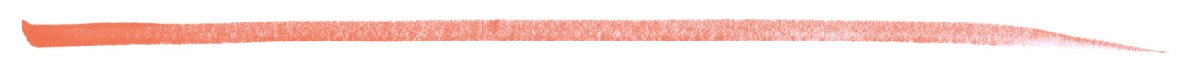
\includegraphics[width=\textwidth]{bar.eps}

\section{Pause}

\begin{description}
\item[Syntax] \verb"\advipause"
\item[Effect] Stop the DVI command rendering at its occurrence.
\end{description}

\begin{minipage}[t]{0.5\textwidth}
\begin{alltt}
Please hit space!{\color{blue}\verb"\"advipause}\verb"\\"
Ok, let's continue.
\end{alltt}
\end{minipage}
\begin{minipage}[t]{0.5\textwidth}
Please hit space!\\ \advipause Ok, let's continue.
\end{minipage}

\section{Wait}

\begin{description}
\item[Syntax] \verb"\adviwait["{\em{sec}}\verb"]"
\item[Effect] Delay the DVI command rendering for {\em{sec}} seconds.
\item[Note] Due to the interval timer calls in the graphics library,\\
  the delay tends to be longer than the specified {\em{sec}} seconds.
\end{description}

\begin{minipage}[t]{0.5\textwidth}
\begin{alltt}
Let's animate a bit.\verb"\advipause\\"
Un,{\color{blue}\verb"\adviwait[1.5]"}
Deux,{\color{blue}\verb"\adviwait[1.5]"}
Trois{\color{blue}\verb"\adviwait{1.5]"}!! 
\end{alltt}
\end{minipage}
\begin{minipage}[t]{0.5\textwidth}
Let's animate a bit.\advipause\\
Un,\adviwait[1.5]
Deux,\adviwait[1.5]
Trois\adviwait[1.5]!! 
\end{minipage}

\section{Record and Play -- Color change}

\begin{description}
\item[Syntax] \verb"\advirecord[play]{"{\em{this}}\verb"}{"{\em{txt}}\verb"}"
\item[Effect] Associates the DVI commands within {\em{txt}} to
  the {\ActiveDVI} tag {\em{this}}.
\item[Note] This macro is used to change the color of {\em{txt}}
later,\\
 with the combination of the \verb"\textcolor" macro.\\
  The scope of the tag is restricted to the current page.\\
  By using the \verb"\advirecord[play]{}{}" macro with the same tag name\\
  more than once, different parts of the page can be associated to the same tag.
\item[Bug] If the tagged text {\em{txt}} contains other tag related
 commands inside, they are ignored.
\end{description}

\begin{description}
\item[Syntax] \verb"\textcolor{" {\em{color}} \verb"}{\adviplay"
                      {\em{this}} \verb"}}"
\item[Effect] Change the color of the texts associated to the tag {\em{this}}.
\item[Note] You need to use the style \verb"color.sty" from the
\verb"graphics" {\LaTeX} package.
\end{description}

\noindent
\begin{minipage}[t]{0.5\textwidth}
\begin{alltt}
{\color{blue}\verb"\advirecord[play]{red}{Red}"},
{\color{blue}\verb"\advirecord[play]{green}{Green}"}, and
{\color{blue}\verb"\advirecord[play]{blue}{Blue}"} are
{\color{blue}\verb"\advirecord[play]{red}{Rouge}"},
{\color{blue}\verb"\advirecord[play]{green}{Vert}"}, and
{\color{blue}\verb"\advirecord[play]{blue}{Bleu}"} in French.
\verb"\bigskip"
Difficult to remember ?
Then, hit space!\verb"\advipause"
{\color{blue}\verb"\textcolor{red}{\adviplay{red}}"}
{\color{blue}\verb"\textcolor{green}{\adviplay{green}}"}
{\color{blue}\verb"\textcolor{blue}{\adviplay{blue}}"}
\end{alltt}
\end{minipage}\advipause
\begin{minipage}[t]{0.5\textwidth}
\advirecord[play]{red}{Red},
\advirecord[play]{green}{Green}, and
\advirecord[play]{blue}{Blue} are
\advirecord[play]{red}{Rouge},
\advirecord[play]{green}{Vert}, and
\advirecord[play]{blue}{Bleu} in French.\advipause

\bigskip
Difficult to remember ?
Then, hit space!\advipause
\textcolor{red}{\adviplay{red}}
\textcolor{green}{\adviplay{green}}
\textcolor{blue}{\adviplay{blue}}
\end{minipage}

\bigskip
\noindent
Easy, no ? Hit space to continue!\advipause

\section{Record and Play -- Hiding}

\begin{description}
\item[Syntax]  \verb"\advirecord{"{\em{this}}\verb"}{"{\em{txt}}\verb"}"
\item[Effect] The DVI commands are associated to the tag {\em{this}}\\
  as with the macro call \verb"\advirecord[play]{"{\em{this}}\verb"}{"{\em{txt}}\verb"}",\\ 
  but the {\em{txt}} text argument is not rendered.
\item[Note] The hidden text can be displayed later by calling the\\
  \verb"\adviplay" macro.
\item[Bug] If the tagged text {\em{txt}} contains other tag related
  commands inside, they are ignored.
\end{description}

\begin{alltt}
\verb"\begin{tabular}[t]{cccc}"
\verb"  One & " {\color{blue}\verb"\advirecord{tag2}{Two}"} \verb" &" {\color{blue}\verb"\advirecord{tag3}{Three}"} \verb"%"
\verb"      & Caml" {\color{blue}\verb"\advirecord{tag2}{s}"} \verb"\\"
\verb"  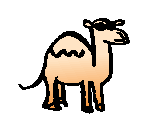
\includegraphics[width=0.1\textwidth]{../tex/caml.eps}&"
\verb" " {\color{blue}\verb"\advirecord{tag2}"}
\verb"   " {\color{blue}\verb"{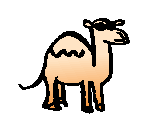
\includegraphics[width=0.1\textwidth]{../tex/caml.eps}}"} \verb"}&"
\verb" " {\color{blue}\verb"\advirecord{tag3}"}
\verb"   " {\color{blue}\verb"{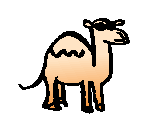
\includegraphics[width=0.1\textwidth]{../tex/caml.eps}}"} \verb"}"
\verb"\end{tabular}"
\color{blue}\verb"\advipause"
\verb"\adviplay{tag2}"
\verb"\advipause"
\verb"\adviplay{tag3}"
\end{alltt}
\begin{tabular}[t]{cccc}
  One & \advirecord{tag2}{Two} & \advirecord{tag3}{Three} & Caml\advirecord{tag2}{s}\\
  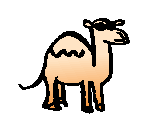
\includegraphics[width=0.1\textwidth]{../tex/caml.eps}&
  \advirecord{tag2}{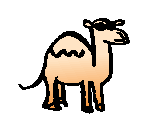
\includegraphics[width=0.1\textwidth]{../tex/caml.eps}}&
  \advirecord{tag3}{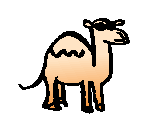
\includegraphics[width=0.1\textwidth]{../tex/caml.eps}}
\end{tabular}
\advipause
\adviplay{tag2}
\advipause
\adviplay{tag3}

\end{document}

% Style.
\renewcommand{\emph}[1]{\textbf{#1}}
\gdef\menhirversion{20200619}


% ------------------------------------------------------------------------------
% Headings.

\title{Visitors\\\normalsize version \visitorsversion}
\date{}
\begin{document}
\author{François Pottier\\ Inria Paris\\ \email{francois.pottier@inria.fr}}
\maketitle

% ------------------------------------------------------------------------------

\clearpage
\tableofcontents
\clearpage

% ------------------------------------------------------------------------------

\begin{flushright}
  Les visites font toujours plaisir, si ce n'est en arrivant, du moins en
  partant. \\ --- \textit{Jean de La Bruyère}
\end{flushright}

\vspace{8mm}

% ------------------------------------------------------------------------------
% ------------------------------------------------------------------------------

\section{Introduction}
\label{sec:intro}

% ------------------------------------------------------------------------------

\subsection{What is a visitor?}

A visitor class for a data structure is a class whose methods implement a
traversal of this data structure. By default, the visitor methods do not have
interesting behavior: they just cause control to go down into the data
structure and come back up, without performing any actual computation.
Nevertheless, by defining subclasses where one method or a few methods are
overridden, nontrivial behavior can be obtained. Therefore, visitors allow
many operations on this data structure to be defined with little effort.

Visitor classes come in several varieties. An \iter visitor traverses a data
structure and returns no result. It can nevertheless have side effects,
including updating a piece of mutable state, raising an exception, and
performing input/output. A \map visitor traverses a data structure and returns
another data structure: typically, a copy of its argument that has been
transformed in some way. An \mapendo visitor is a variant of a \map visitor
that preserves physical sharing when possible. A \reduce visitor traverses a
data structure and returns a value that somehow summarizes it: computing the
size of a data structure is a typical example. A \mapreduce visitor performs
the tasks of a \map visitor and a \reduce visitor at the same time,
possibly allowing symbiosis between them. All of these can be viewed as
special cases of the \fold visitor, which performs a bottom-up computation
over a data structure. The class \fold is equipped with virtual methods
% (the ``\tyconascendingmethod{}'' methods)
that can be overridden (in a subclass) so as to specify what computation is
desired.

Visitors also come in several arities. The visitors mentioned above have arity
one: they traverse one data structure. However, it is sometimes necessary to
simultaneously traverse two data structures of identical shape. For this
purpose, there are visitors of arity two: here, they are known as \itertwo,
\maptwo, \reducetwo, \mapreducetwo, and \foldtwo visitors.

% \mapendotwo does not exist.

% ------------------------------------------------------------------------------

\subsection{What does this package offer?}

Visitors have extremely regular structure. As a result, whereas implementing
them by hand is boring and error-prone, generating them automatically is often
possible. The \visitors package extends the syntax of OCaml%
%
\footnote{Technically, \visitors is a plugin for \ppxderiving, which itself is
  a preprocessor extension for the OCaml compiler.}
%
so as to make it easy for the programmer to request the automatic generation
of visitor classes. Visitor classes for many forms of user-defined data types
can be generated and, if necessary, combined (via multiple inheritance) with
hand-written visitor classes, making the framework quite powerful.

% ------------------------------------------------------------------------------
% ------------------------------------------------------------------------------

\section{Walkthrough}

% ------------------------------------------------------------------------------

\subsection{Setup}
\label{sec:intro:setup}

\enlargethispage{\baselineskip}

In order to install the \visitors package, an \opam user should issue the
following commands:
\begin{lstlisting}[keywords={}]
  opam update
  opam install visitors
\end{lstlisting}
To use the package, an \ocamlbuild user should add the
following line in her project's \texttt{\_tags} file:
\begin{lstlisting}[keywords={}]
  true: package(visitors.ppx)
\end{lstlisting}
while a user of \dune should add the following incantation
to her project's \texttt{dune} file,
inside a \texttt{library} or \texttt{executable} stanza:
\begin{lstlisting}[keywords={}]
  (preprocess (pps visitors.ppx))
\end{lstlisting}
%% A user of \merlin should add the following lines in her project's
%% \texttt{.merlin} file:
%% \begin{lstlisting}[keywords={}]
%%   PKG visitors.ppx
%% \end{lstlisting}
To use the \visitors package in OCaml's interactive ``toplevel'' environment,
launch \texttt{ocaml} and type the following commands:
\begin{lstlisting}
  #use "topfind";;
  #require "visitors.ppx";;
\end{lstlisting}

% ------------------------------------------------------------------------------

\begin{figure}[t]
% In an OCaml source file, a type definition can be annotated with
% \derivingvisitors:
\orig{expr00}
% This causes the following code to be (invisibly) generated:
\vspace{-\baselineskip}
\processed{expr00}
\caption{A visitor of the \iter variety}
\label{fig:expr00}
\end{figure}

\subsection{Defining an \iter visitor}
\label{sec:intro:iter:def}

Suppose we need to manipulate arithmetic expressions built out of integer
literals and binary additions. The abstract syntax of these expressions can be
described by an algebraic data type \oc|expr|, shown in the first part of
\fref{fig:expr00}.
%
By annotating this type definition with \derivingvisitors, we request the
automated generation of a visitor for expressions. The annotation
\derivingvisitors must carry at least one parameter, \variety, which indicates
what variety of visitor is desired.

The code of the visitor class, which is automatically generated and in normal
use remains invisible, is shown in the second part of \fref{fig:expr00}. The
name of this class is by default the value of the \variety parameter. It can
be changed, if desired, by explicitly supplying a \name parameter.

A visitor takes the form of an OCaml class, whose methods are named after the
types and data constructors that appear in the type definition. In
\fref{fig:expr00}, for instance, the method \tyconvisitor{expr} is named after
the type \oc|expr|, while the methods \dataconvisitor{EConst} and
\dataconvisitor{EAdd} are named after the data constructors \oc|EConst| and
\oc|EAdd|.

Different varieties of visitors differ in the computation that is performed
``on the way up'', after the recursive calls have finished, therefore differ
in the return types of the visitor methods. \iter is the simplest variety. An
\iter visitor performs no computation on the way up, so its methods have
return type \oc|unit|.

In an \iter visitor, the generated visitor methods do nothing. In
\fref{fig:expr00}, for instance, the method \tyconvisitor{expr} inspects its
argument \oc|this| and recursively invokes either \dataconvisitor{EConst} or
\dataconvisitor{EAdd}, as appropriate. The method \dataconvisitor{EConst} does
nothing.\footnote{More precisely, it calls the method \tyconvisitor{int},
  which is inherited from the class \runtime{iter}, and does
  nothing. This call to \tyconvisitor{int} can be avoided, if desired, by using
  \oc|(int[@opaque])| instead of \oc|int|; see \sref{sec:opaque}.} The method
\dataconvisitor{EAdd} performs two recursive calls to \tyconvisitor{expr},
which does nothing, so \dataconvisitor{EAdd} itself does nothing.

Every method is parameterized with an environment \oc|env|, which is carried
down into every recursive call and is otherwise unused. The type of this
environment is undetermined: it is up to the (user-defined) subclasses of the
visitor class to decide what the type of \oc|env| should be and (possibly)
where and how this environment should be enriched.

% One could note that the visitor class is parameterized over 'self,
% but it is perhaps a bit early for such a remark.

The fields of a data constructor or record are traversed left to right, in the
order they are declared. In a list-like data structure, the field that holds a
pointer to the list tail should be declared last, so as to ensure that the
traversal requires constant stack space.

% ------------------------------------------------------------------------------

\begin{figure}[t]
\codefollowup{expr00}
\origfirstline{expr04}{3}
\caption{Counting the number of addition nodes in an expression}
\label{fig:expr04}
\end{figure}

\subsection{Using an \iter visitor}
\label{sec:intro:iter:usage}

Naturally, traversing a data structure without actually computing anything is
not a very sensible thing to do. Things become interesting when at least one
visitor method is overridden so as to give rise to nontrivial behavior.
Suppose, for instance, that we wish to count the number of addition nodes in
an expression. This can be done as shown in \fref{fig:expr04}. We create an
object~\oc|v| that is both a counter (that is, an object equipped with a
mutable field~\oc|count|) and a visitor, and we override its method
\dataconvisitor{EAdd} so that the counter is incremented every time this
method is invoked. There remains to run the visitor, by invoking its
\tyconvisitor{expr} method, and to return the final value of the counter. The
environment, in this example, is unused; we let it have type \unit.

This may seem a rather complicated way of counting the addition nodes in an
expression. Of course, one could give a direct recursive definition of the
function \oc|count|, in a few lines of code, without using a visitor at all.
The point of employing a visitor, as done in Figures~\ref{fig:expr00}
and~\ref{fig:expr04}, is that no changes to the code are required when the
type of expressions is extended with new cases.

% ------------------------------------------------------------------------------

\subsection{What is the type of a visitor?}
\label{sec:intro:type}

In this document, most of the time, we prefer to show the code of a visitor
class and omit its type. There are two reasons for this. First, this type is
often verbose, as the class has many methods, and complex, as several type
variables are often involved. Second, although we can explain the type of a
generated visitor on a case-by-case basis, we cannot in the general case
predict the type of a generated visitor.
The reason is, the type of a generated visitor depends upon the
types of the classes that are inherited via the \ancestors parameter
(\sref{sec:ancestors}). Because a \texttt{ppx} syntax extension transforms
untyped syntax trees to untyped syntax trees, the \visitors syntax extension
does not have access to this information.

For this reason, the \visitors syntax extension cannot generate any type
declarations. Thus, the annotation \derivingvisitors can be used only in an
\texttt{\%.ml} file, not in an \texttt{\%.mli} file. When it is used in an
\texttt{\%.ml} file, the corresponding \texttt{\%.mli} file should either be
omitted altogether or be written by hand.

\begin{figure}[t]
\begin{mdframed}[backgroundcolor=green!10]
\begin{lstlisting}
class virtual ['self] iter : object ('self)
  constraint 'self =
    < visit_EAdd : 'env -> expr -> expr -> unit;
      visit_EConst : 'env -> int -> unit;
      visit_expr : 'env -> expr -> unit;
      .. >
  method visit_EAdd : 'env -> expr -> expr -> unit
  method visit_EConst : 'env -> int -> unit
  method visit_expr : 'env -> expr -> unit
  (* These methods are inherited from [VisitorsRuntime.iter]: *)
  method private visit_array :
    'env 'a. ('env -> 'a -> unit) -> 'env -> 'a array -> unit
  method private visit_bool : 'env. 'env -> bool -> unit
  method private visit_bytes : 'env. 'env -> bytes -> unit
  (* ... and many more ... *)
end
\end{lstlisting}
\end{mdframed}
\caption{An inferred type for the \iter visitor of \fref{fig:expr00}}
\label{fig:inferred}
\end{figure}

\begin{figure}[t]
\begin{mdframed}[backgroundcolor=green!10]
\begin{lstlisting}
class virtual ['self] iter : object ('self)
  method visit_EAdd   : 'monomorphic. 'env -> expr -> expr -> unit
  method visit_EConst : 'monomorphic. 'env -> int -> unit
  method visit_expr   : 'monomorphic. 'env -> expr -> unit
end
\end{lstlisting}
\end{mdframed}
\caption{A simplified type for the \iter visitor of \fref{fig:expr00}}
\label{fig:simplified}
\end{figure}


Nevertheless, the type of the generated code can be inspected, if desired, by
requesting the OCaml compiler to infer and display it. For this purpose, one
can use a command of the following form:
\begin{quote}
\verb|ocamlbuild -use-ocamlfind <other-flags> %.inferred.mli|
\end{quote}

\fref{fig:inferred} shows the type that is inferred via such a command for the
\iter visitor of \fref{fig:expr00}. This type is rather verbose, for two
reasons. First, an explicit type equation, introduced by the \oc|constraint|
keyword, relates the type parameter \oc|'self| with an OCaml object type that
lists the public methods with their types. Second, the class \iter has many more
methods than one might think. This is because it inherits a large number of
private methods from the class \runtime{iter}. In the present case, all of
these methods except \tyconvisitor{int} are in fact unused.

Fortunately, this complicated type can be manually simplified. This is done in
\fref{fig:simplified}. Two main simplifications have been performed. First, we
have omitted all private methods. Indeed, the most important property of
private methods in OCaml is precisely the fact that it is permitted to hide
their existence. Second, we have omitted the type constraint that bears on
the type variable \oc|'self|, as it is in fact redundant: it is implicit in OCaml
that the type of ``self'' must be an object type that lists the public methods.
The bizarre-looking ``\oc|'monomorphic.|'' annotations indicate that the methods have
monomorphic types. (This notational trick is explained in \sref{sec:oo:monomorphic}.)
This means that the type variable~\oc|'env| is not quantified at the level of each
method\footnote{That would be undesirable, as it would force each method to
treat the environment as an argument of unknown type!}, but at the level of the class.
This means that the three methods must agree on the type of the environment, and
that this type is presently undetermined, but can be determined in a subclass.

The class type shown in \fref{fig:simplified} cannot be further simplified.
The methods \tyconvisitor{EConst} and \tyconvisitor{EAdd} cannot be hidden, as
they are public. That said, if one wished to hide them, one could add the parameter %
\oc|public = ["visit_expr"]| to the annotation \derivingvisitors in \fref{fig:expr00}.
These two methods would then be declared private in the generated code,
so it would be permitted to hide their existence.

Although we have claimed earlier that one cannot in the general case predict
the type of a generated visitor method, or even predict whether a generated
method will be well-typed, it is possible to define a convention which in many
cases can be adhered to. This convention is presented later on
(\refconvention).

% ------------------------------------------------------------------------------

\begin{figure}[t]
\orig{expr01}
\vspace{-\baselineskip}
\processed{expr01}
\caption{A visitor of the \map variety}
\label{fig:expr01}
\end{figure}

\subsection{\map visitors}
\label{sec:intro:map}

An \iter visitor returns no result. Although, as illustrated previously
(\sref{sec:intro:iter:usage}), it can use private mutable state to accumulate
information, there are applications for which such a visitor is not suitable.
One class of such applications is tree transformations. To transform an
expression into an expression, one should use a visitor of another variety,
namely \map.

A \map visitor is shown in \fref{fig:expr01}. In comparison with the \iter
visitor of \fref{fig:expr00}, the generated code is identical, except that,
instead of returning the unit value \oc|()|, the method
\dataconvisitor{EConst} reconstructs an \oc|EConst| expression, while the
method \dataconvisitor{EAdd} reconstructs an \oc|EAdd| expression.

A \map visitor behaves (by default) as an identity function: it constructs a
copy of the data structure that it visits. If the data structure is immutable,
this is rather pointless: in order to obtain nontrivial behavior, at least one
method should be overridden. If the data structure is mutable, though, even
the default behavior is potentially of interest: it constructs a deep copy of
its argument.

% ------------------------------------------------------------------------------

\begin{figure}[p]
\orig{expr00endo}
\vspace{-\baselineskip}
\processed{expr00endo}
\caption{A visitor of the \mapendo variety}
\label{fig:expr00endo}
\end{figure}

\subsection{\mapendo visitors}
\label{sec:intro:endo}

\mapendo visitors are a slight variation of \map visitors. Whereas a \map
visitor systematically allocates a copy of the memory block that it receives
as an argument, an \mapendo visitor (\fref{fig:expr00endo}) first tests if the
newly allocated block would have exactly the same contents as the original
block, and if so, re-uses the original block instead.
% Didier attributes this idea to Gérard Huet,
% at least in the case of a dictionary insertion operation,
% where Gérard would raise an exception so as to go back to
% the toplevel and avoid re-allocating a path.
%
This trick allows saving memory: for instance, when a performing a
substitution operation on a term, the subterms that are unaffected
by the substitution are not copied.

One potential disadvantage of \mapendo visitors, in comparison with \map
visitors, is that these runtime tests have a runtime cost. A more serious
disadvantage is that \mapendo visitors have less general types: in an \mapendo
visitor, the argument type and return type of every method must coincide,
whence the name ``\mapendo''.
%
(An endomorphism is a function of a set into itself.)
%
\map visitors are not subject to this restriction: for an illustration, see
\sref{sec:advanced:hashconsed} and \fref{fig:expr14}.

In principle, \mapendo visitors should be created only for immutable data
structures. Although the tool can produce an \mapendo visitor for a mutable
data structure, this is discouraged, as it may lead to unexpected behavior.

% ------------------------------------------------------------------------------

\begin{figure}[p]
\orig{expr15}
\vspace{-\baselineskip}
\processed{expr15}
\caption{A visitor of the \reduce variety}
\label{fig:expr15}
\end{figure}

\begin{figure}[t]
\codefollowup{expr15}
\origfirstline{expr15b}{3}
\caption{Computing the size of an expression using a \reduce visitor}
\label{fig:reduce}
\end{figure}

\subsection{\reduce visitors}
\label{sec:intro:reduce}

Whereas an \iter visitor returns no result and a \map visitor returns a data
structure, a \reduce visitor returns a ``summary'' of a data structure, so to
speak. The summary of a term is computed by combining the summaries of its
subterms. This requires summaries to inhabit a monoid, that is, a type
equipped with a binary operation \oc|plus| and its neutral element \oc|zero|.

\fref{fig:expr15} shows a \reduce visitor for arithmetic expressions. In
\dataconvisitor{EAdd}, the summaries produced by the two recursive calls are
combined using a call to \oc|self#plus|. In \dataconvisitor{EConst}, there are
no recursive calls, so there is nothing to combine: the result is
\oc|self#zero|.

The virtual methods \oc|zero| and \oc|plus| are declared in the class
\runtime{reduce}, which is automatically inherited. The type of the
monoid elements, at this point, is undetermined: it is up to the
(user-defined) subclasses of the class \reduce to decide what this type should
be and what the monoid operations should be.

As an example application, \fref{fig:reduce} shows how to compute the size of
an expression using a \reduce visitor. We inherit the class \reduce. We also
inherit the class \runtime{addition_monoid}, which defines the
methods \oc|zero| and \oc|plus| as the integer \oc|0| and integer addition,
respectively. There remains to override the method \tyconvisitor{expr} so as
to indicate that every node contributes 1 to the size of an expression.

Incidentally, this code is written in such a manner that a single visitor
object is created initially and serves in every call to the function
\oc|size|. This style can be used when the visitor object is immutable and
when the function that one wishes to define is monomorphic. When it cannot be
used, one begins with \oc|let size (e : expr) : int = ...| and ends with %
\oc|v # visit_expr () e|. That style causes a new visitor object to be created
every time \oc|size| is called.
% On pourrait ré-utiliser le même objet à chaque fois en remettant son champ à
% zéro... Mais ce serait sale et pas ré-entrant.

The size of an expression can also be computed using an \iter visitor equipped
with mutable state, in the style of \fref{fig:expr04}. It is mostly a matter
of style whether such a computation should be performed using \iter or
\reduce.
% TEMPORARY comparer les perfs, pour voir

An \iter visitor is in fact a special case of a \reduce visitor, instantiated
with the \oc|unit| monoid. Thus, in principle, one could forget \iter and
always work with \reduce. Nevertheless, it is preferable to work with \iter
when it is applicable, for reasons of clarity and efficiency.
% e.g. an \iter visitor can traverse a list-like data structure in constant
% stack space; a \reduce visitor cannot, because it does not have an accu.

% One might wonder whether a reduce visitor should have an accumulator...
% ...but then it would be left-to-right-from-the-start, instead of bottom-up.
% I am not sure what we want. Maybe we do not need reduce visitors at all!

% ------------------------------------------------------------------------------

\begin{figure}[p]
\orig{expr_info_mapreduce}
\vspace{-\baselineskip}
\processed{expr_info_mapreduce}
\caption{A visitor of the \mapreduce variety}
\label{fig:mapreduce}
\end{figure}

\begin{figure}[p]
\codefollowup{mapreduce}
\origfirstline{expr_info_mapreduce_use}{3}
\caption{Decorating every subexpression with its size}
\label{fig:expr_info_mapreduce_use}
\end{figure}

\subsection{\mapreduce visitors}
\label{sec:intro:mapreduce}

A \mapreduce visitor performs the tasks of a \map visitor and a \reduce
visitor at once. An example appears in \fref{fig:mapreduce}. Every visitor
method returns a pair of a transformed term and a summary. In other words,
it returns a pair of the results that would be returned by a \map visitor
method and by a \reduce visitor method.

Like a \reduce visitor, a \mapreduce visitor performs a bottom-up computation.
Like a \map visitor, it constructs a new tree. By default, these two tasks are
independent of one another. However, by overriding one or more methods, it is
easy to establish a connection between them: typically, one wishes to exploit
the information that was computed about a subtree in the construction of the
corresponding new subtree. As an example, \fref{fig:expr_info_mapreduce_use}
shows how to transform an arithmetic expression into an arithmetic expression
where every subexpression is annotated with its size. (This example uses a
parameterized type of decorated expressions, which is explained in
\sref{sec:intro:parameterized:mono}. We suggest reading the explanations there
first.) The transformation is carried out in one pass and in linear time. As
in \fref{fig:reduce}, we use the addition monoid to compute integer sizes.
This time, however, the visitor methods return not just a size, but a pair of
a new expression and a size. The method \tyconvisitor{expr} is overridden so
as to store the size of the subexpression, \oc|size|, in the \oc|info| field
of the new expression. Because the overridden method \tyconvisitor{expr} does
not call \tyconvisitor{'info}, the latter method is never called: we provide a
dummy definition of it.

Other example applications of \mapreduce visitors include:
\begin{itemize}[nosep]
\item decorating every subterm of a $\lambda$-term with the set of its free
  variables;
\item decorating every internal node of abstract syntax tree with a region in
  the source code (assuming that every leaf carries such a region already).
\end{itemize}

% ------------------------------------------------------------------------------

\begin{figure}[p]
\orig{expr00fold}
\vspace{-\baselineskip}
\processed{expr00fold}
\caption{A visitor of the \fold variety}
\label{fig:expr00fold}
\end{figure}

\begin{figure}[p]
\orig{fold}
\caption{Converting towards unrelated types using a \fold visitor}
\label{fig:fold}
\end{figure}

\subsection{\fold visitors}
\label{sec:intro:fold}

The varities of visitors presented up to this point differ in the computation
that they perform on the way up, after the recursive calls. As we have seen,
\iter visitors perform no computation at all; \map and \mapendo visitors
reconstruct a term; \reduce visitors perform a series of monoid operations.
Each variety follows a baked-in pattern, which has been programmed ahead of
time, and cannot be changed. What if a different form of computation, which
has not been envisioned by the author of the \visitors syntax extension, is
needed?

This is where \fold visitors come in. A \fold visitor declares virtual methods
that are called on the way up and can be overridden by the user (in a
subclass) so as to implement the desired computation. \fref{fig:expr00fold}
shows a \fold visitor. Two virtual methods, \dataconascendingmethod{EConst}
and \dataconascendingmethod{EAdd}, are declared. They are invoked by
\tyconvisitor{EConst} and \tyconvisitor{EAdd}, respectively.

In a \fold visitor, the return type of the visitor methods is not fixed ahead
of time. It is up to the (user-defined) subclasses of the visitor class to
decide what this type should be.

As an example application, \fref{fig:fold} shows how a \fold visitor can be
used to convert the visited data structure to an entirely different format. In
this example, the type \oc|person| is a record type, whose fields are
\oc|firstname| and \oc|surname|. The type \oc|crowd| is isomorphic to a list
of persons, but, for some reason, it is declared as an algebraic data type
equipped with its own data constructors, \oc|Nobody| and \oc|Someone|. Suppose
we wish to convert a \oc|crowd| to a list of pairs of strings. We can do so by
creating a visitor object that inherits the class \fold and provides concrete
implementations of the methods \tyconascendingmethod{person},
\dataconascendingmethod{Nobody}, and \dataconascendingmethod{Someone}.
Our implementation of \tyconascendingmethod{person} simply allocates
a pair, while our implementations of
\dataconascendingmethod{Nobody} and \dataconascendingmethod{Someone}
respectively build an empty list and a nonempty list.
Thus, the return type of the methods \tyconascendingmethod{person}
and \tyconvisitor{person} is \oc|string * string|,
while the return type of the methods \dataconascendingmethod{Nobody},
\dataconascendingmethod{Someone}, and \dataconvisitor{crowd} is
\oc|(string * string) list|. In a \fold visitor, not all methods
need have the same return type!

If we had chosen to return \oc|f ^ s| instead of \oc|(f, s)| in
\tyconascendingmethod{person}, then a crowd would be converted to
a \oc|string list|. A \fold visitor offers great flexibility.

All previous varieties of visitors are special cases of \fold visitors. The
specialized varieties of visitors are more convenient to use, when they can be
used, because they do not require the user to provide \tyconascendingmethod{}
methods. Yet, \fold visitors are in principle more versatile.%
%
\footnote{This would be true in an untyped setting, but is not quite true in OCaml,
due to restrictions imposed by OCaml's type discipline (\sref{sec:map_from_fold}).}

% ppx_tools/genlifter is analogous, with a few differences:
% - it is a command line tool, not as ppx extension;
% - it has only one return type 'res for all methods;
% - the visitor methods receive (as extra arguments)
%   the names of the types, data constructors, and record fields
%   that are being visited.
% - and there are fewer visitor methods, basically one per type,
%   plus one primitive type, plus this#record, this#constr.

% TEMPORARY show how to do a fold in the presence of primitive types, e.g., list
% writing ancestors = ["VisitorsRuntime.map"] may be necessary

% ------------------------------------------------------------------------------

\begin{figure}[p]
\orig{expr02}
\vspace{-\baselineskip}
\processed{expr02}
\caption{A visitor of the \itertwo variety}
\label{fig:expr02}
\end{figure}

\begin{comment}
\begin{figure}[p]
\orig{expr03}
\vspace{-\baselineskip}
\processed{expr03}
\caption{A visitor of the \maptwo variety}
\label{fig:expr03}
\end{figure}
\end{comment}

\subsection{Visitors of arity two}
\label{sec:intro:aritytwo}

The visitors introduced so far traverse one tree at a time. There are
situations where one wishes to simultaneously traverse two trees, which one
expects have the same structure. For this purpose, one can use a visitor of
arity 2. Every variety except \mapendo is available at arity 2.

As an illustration, \fref{fig:expr02} shows an \itertwo visitor. There, the
method \tyconvisitor{expr} expects an environment and two expressions. These
expressions must have identical structure: indeed, if \tyconvisitor{expr}
finds that they exhibit different tags at the root, say \oc|EConst| versus
\oc|EAdd|, then it invokes the method \tyconfail{expr}, whose default
implementation calls the function \runtime{fail}. This function
throws the exception \runtime{StructuralMismatch}.

In \fref{fig:expr02}, we have added the optional parameter
%
\oc|concrete = true|
%
to indicate that the generated class should not be virtual. (By default,
every generated class is declared \oc|virtual|.) We do this because, in
the illustration that follows, we wish to instantiate this class.

\begin{figure}[p]
\codefollowup{expr02}
\origfirstline{expr05}{3}
\caption{Determining whether two expressions are syntactically equal}
\label{fig:expr05}
\end{figure}

\begin{figure}[p]
\codefollowup{expr02}
\origfirstline{expr05lexico}{3}
\caption{Determining which way two expressions are ordered}
\label{fig:expr05lexico}
\end{figure}

As an illustration, in \fref{fig:expr05}, we use an \itertwo visitor to write
a function that tests whether two expressions are syntactically equal. This is
just a matter of performing a synchronous traversal of the two expressions and
detecting a \oc|StructuralMismatch| exception: if this exception is raised,
one must return \oc|false|, otherwise one must return \oc|true|. We rely on
the fact that the method \tyconvisitor{int}, which is inherited from the class
\runtime{iter2}, fails when its two integer arguments are
unequal.

The convenience functions \runtime{wrap} and
\runtime{wrap2} run a user-supplied function (of arity 1 or 2,
respectively) within an exception handler and return a Boolean result, which
is \oc|true| if no exception was raised. Here, we run the function
%
\oc|new iter2 # visit_expr ()|, whose type is \oc|expr -> expr -> unit|,
in the scope of such a handler.

Naturally, to test whether two expressions are syntactically equal, one could
also use the primitive equality operator \oc|=|. Alternatively, one could
exploit \ppxderiving and annotate the type definition with
%
\oc|[@@deriving eq]|. Visitors offer greater flexibility: for instance, if our
arithmetic expressions contained variables and binders, we could easily define
an operation that tests whether two expressions are $\alpha$-equivalent.

As a second illustration, in \fref{fig:expr05lexico}, we use an \itertwo
visitor to write a lexicographic ordering function for expressions. Again,
this involves a synchronous traversal of the two expressions. When a mismatch
is detected, however, one must not raise a \oc|StructuralMismatch| exception:
instead, one must raise an exception that carries one bit of information,
namely, which of the two expressions is strictly ``smaller'' in the ordering.
The exception \oc|Different| is introduced for this purpose; it carries an
integer return code, which by convention is either -1 or +1. Two visitor methods
must be overridden, namely \tyconvisitor{int}, which is in charge of detecting
a mismatch between two integer constants, and \tyconfail{expr}, which is invoked
when a mismatch between (the head constructors of) two expressions is detected.
The auxiliary function \oc|tag| returns an integer code for the head constructor
of an expression. It must be hand-written. One could in principle write such a
function once and for all by using the undocumented operations in OCaml's
\href{https://caml.inria.fr/pub/docs/manual-ocaml/libref/Obj.html}{\oc|Obj|}
module, but that is discouraged.

% Il faut au minimum distinguer les constructeurs constants des autres,
% en utilisant is_int. Il y a peut-être d'autres pièges. De plus, on ne
% peut pas (je crois?) garantir que l'ordre des constructeurs sera bien
% celui de la déclaration de types, parce que les constructeurs constants
% et les autres sont codés indépendamment.

% ------------------------------------------------------------------------------

\begin{figure}[t]
\orig{expr06}
\caption{Visitors for a family of types}
\label{fig:expr06}
\end{figure}

\subsection{Visitors for a family of types}
\label{sec:intro:family}

Visitors can be generated not just for one type definition, but for a family
of type definitions. In \fref{fig:expr06}, we propose a definition of
arithmetic expressions that involves three algebraic data types, namely
\oc|unop|, \oc|binop|, and \oc|expr|. We request the generation of two
visitors, namely an \iter visitor and a \map visitor. This causes the
generation of just two classes, named \iter and \map, respectively. Each of
these classes has visitor methods for every type (namely \tyconvisitor{unop},
\tyconvisitor{binop}, \tyconvisitor{expr}) and for every data constructor
(namely \dataconvisitor{UnaryMinus}, \dataconvisitor{BinaryMinus}, and so on).

Note that, for the \derivingvisitors annotation to apply to the entire family,
as opposed to just the type \oc|expr|, the types \oc|unop|, \oc|binop|, and
\oc|expr| in \fref{fig:expr06} are declared simultaneously: that is, their
declarations are separated with the keyword \oc|and|.

% ------------------------------------------------------------------------------

\subsection{Visitors for parameterized types}
\label{sec:intro:parameterized}

% ------------------------------------------------------------------------------

Visitors can be generated for parameterized types, too. However, there are two
ways in which this can be done. Here is why.

To visit a data type where some type variable~\oc|'a| occurs, one must know
how to visit a value of type~\oc|'a|.
%
% That is not quite true, in reality: perhaps there is no component of
% type~\oc|'a|, perhaps because \oc|'a| is a phantom type parameter or a GADT index,
% or perhaps because \oc|'a| occurs only under a type constructor that performs
% special treatment and does not recursively descend its own components.
%
There are two ways in which this information can be provided. One way is to
assume that there is a \emph{virtual visitor method} \oc|visit_'a| in charge
of visiting a value of type~\oc|'a|. Another way is to pass a \emph{visitor
  function} \oc|visit_'a| as an argument to every visitor method.

% J'allais écrire que dans un cadre non typé, ces deux approches ont la
% même expressivité. Mais c'est faux: seule la seconde approche permet
% de gérer les types de données non réguliers (qui existent aussi dans
% un cadre non typé, même s'ils ne sont pas explicitement décrits par
% une déclaration).

These two approaches differ in their expressive power. The
virtual-visitor-method approach implies that the visitor methods must have
monomorphic types: roughly speaking, the type variable~\oc|'a|
% (or variants of it)
appears free in the type of every visitor method.
The visitor-function approach implies that the visitor methods can have
polymorphic types: roughly speaking, each method independently
can be polymorphic in \oc|'a|.
For this reason, we refer to these two approaches as the \emph{monomorphic}
approach and the \emph{polymorphic} approach, respectively.

The monomorphic approach offers the advantage that the type of every method is
inferred by OCaml. Indeed, in this mode, the generated code need not contain
any type annotations. This allows correct, most general (monomorphic) types to
be obtained even in the case where certain hand-written visitor methods
(provided via the \ancestors parameter) have unconventional types.
%
% The downside of this approach is that it does not allow taking several
% distinct instances of a parameterized type. In particular, it is restricted
% to regular algebraic data types (\sref{sec:regularity}).

The polymorphic approach offers the advantage that visitor methods can receive
polymorphic types. If the type \oc|container| is parameterized with a type
variable~\oc|'a|, then the method \tyconvisitor{container} can be assigned a
type that is universally quantified in~\oc|'a|, of the following form:
%
\begin{mdframed}[backgroundcolor=green!10]
\begin{lstlisting}
method visit_container:
  'env 'a .
  ('env -> 'a -> ...) ->
  'env -> 'a container -> ...
\end{lstlisting}
\end{mdframed}
%
The types of the \tyconvisitor{list} methods, shown later on
(\sref{sec:intro:nonlocal}, \fref{fig:convention}), follow this pattern.
%
Because \tyconvisitor{container} is polymorphic, taking multiple instances of
the type \oc|container|, such as \oc|apple| \oc|container| and \oc|orange|
\oc|container|, and attempting to generate visitor methods for these types,
poses no difficulty. This works even if the definition of \oc|'a container|
mentions other instances of this type, such as \oc|('a * 'a)| \oc|container|.
In other words, in the polymorphic approach, irregular algebraic data types
(\sref{sec:regularity}) are supported.

One downside of the polymorphic approach is that, because polymorphic types
cannot be inferred by OCaml, the \visitors syntax extension must generate
polymorphic type annotations. Therefore, it must be able to predict
the type of every visitor method.
%
% Actually, not the full type, but at least the polymorphic skeleton.
%
This requires that any visitor methods inherited via \ancestors adhere to a
certain convention (\refconvention).

In summary, both the monomorphic approach and the polymorphic approach are
currently supported (\sref{sec:intro:parameterized:mono},
\sref{sec:intro:parameterized:poly}). The parameter \polymorphic allows
choosing between them. As a rule of thumb, we suggest setting
%
\oc|polymorphic = true|, as this produces visitors that compose better.

% TEMPORARY give an explanation why monomorphic mode can be useful?

% In my ICFP paper, I believe monomorphic mode is necessary to deal with ['bn]
% and ['env]. Indeed, we cannot expect [visit_abs] to be polymorphic in ['bn]
% and ['env], as it needs to be told how to [extend] an environment with a
% bound name.

% Other examples?

% ------------------------------------------------------------------------------

\begin{figure}[p]
\orig{expr_info}
\vspace{-\baselineskip}
\processed{expr_info}
\caption{A ``monomorphic-method'' visitor for a parameterized type of decorated expressions}
\label{fig:expr_info}
\end{figure}

\begin{figure}[p]
\codefollowup{expr_info}
\origfirstline{expr_info_use}{3}
\caption{Working with different types of decorations}
\label{fig:expr_info_use}
\end{figure}

\subsubsection{Monomorphic visitor methods for parameterized types}
\label{sec:intro:parameterized:mono}

We begin with an example of the \emph{monomorphic} mode. This mode can be
explicitly requested by writing \oc|polymorphic = false| as part of the
\derivingvisitors annotation. It is the default mode.

In \fref{fig:expr_info}, we define a variant of arithmetic
expressions where every tree node is decorated with a value of type
\oc|'info|. We request the generation of a \map visitor, whose code is shown
in the second part of \fref{fig:expr_info}. The generated code has exactly the
same structure as in the previous sections. The only new feature is that the
class \map now has a virtual method, \tyconvisitor{'info}. The general rule
is, for each type parameter, there is one virtual method, named after it.

The visitor methods are \emph{not} declared polymorphic in a type
variable~\oc|'info|, or in two type variables \oc|'info1|~and~\oc|'info2|, as
one might perhaps expect. In fact, they must not be declared polymorphic:
indeed, the user who implements \tyconvisitor{'info} in a subclass of \map may
wish to provide an implementation that expects and/or produces specific types
of information.

As a result, a visitor \emph{object} is monomorphic: its method
\tyconvisitor{'info} must have type \oc|info1 ->| \oc|info2| for certain
specific types \oc|info1| and \oc|info2|. Fortunately, because it is
parameterized over \oc|'self|,\footnote{We explain in \sref{sec:oo:self} why
  all visitor classes are parameterized over \oc|'self|.} the visitor
\emph{class} is polymorphic: two distinct visitor objects can have distinct
types.

Although every \emph{automatically generated} method
is monomorphic, a visitor class can nevertheless \emph{inherit} polymorphic
methods from a parent class, whose name is specified via the \ancestors parameter
(\sref{sec:ancestors}). For instance, the \tyconvisitor{list} methods provided by
the classes \runtime{iter}, \runtime{map}, and so on, are
polymorphic in the types of the list elements. (See \sref{sec:intro:nonlocal}
for more information on the treatment of preexisting types.)

\fref{fig:expr_info_use} presents two example uses of the class \map defined in
\fref{fig:expr_info}. In the first example, we define a function \oc|strip|, of
type \oc|'info expr -> unit expr|, which strips off the decorations in an
arithmetic expression, replacing them with unit values. In the second example,
we define a function \oc|number|, of type \oc|'info expr -> int expr|, which
decorates each node in an arithmetic expression with a unique integer number.%
\footnote{Because the \oc|info| field appears before the \oc|node| field in
  the definition of the type \oc|expr|, and because fields are visited
  left-to-right, we get a prefix numbering scheme. By exchanging these fields,
  we would get postfix numbering.} %

% ------------------------------------------------------------------------------

\subsubsection{Polymorphic visitor methods for parameterized types}
\label{sec:intro:parameterized:poly}

\begin{figure}[p]
\orig{expr_info_polymorphic}
\vspace{-\baselineskip}
\processed{expr_info_polymorphic}
\caption{A ``polymorphic-method'' visitor for a parameterized type of decorated expressions}
\label{fig:expr_info_polymorphic}
\end{figure}

\begin{figure}[p]
\codefollowup{expr_info_polymorphic}
\origfirstline{expr_info_polymorphic_use}{3}
\caption{Working with different types of decorations}
\label{fig:expr_info_polymorphic_use}
\end{figure}

We continue with an example of the \emph{polymorphic} mode. This mode can be
explicitly requested by writing \oc|polymorphic = true| as part of the
\derivingvisitors annotation. It is available for all varieties of visitors
except \fold and \foldtwo. The reason why it seems difficult to come up with
a satisfactory polymorphic type for \fold visitor methods is explained later
on (\sref{sec:map_from_fold}).

In \fref{fig:expr_info_polymorphic}, we again have arithmetic expressions
where every tree node is decorated with a value of type \oc|'info|. We again
request a \map visitor but, this time, we specify \oc|polymorphic = true|.
%
In order to make the generated code shorter, we specify \oc|data = false|
(\sref{sec:params}), which causes the methods \dataconvisitor{EConst} and
\dataconvisitor{EAdd} to disappear. (They are inlined at their call sites.)

The generated code is the same as in the previous section,
% except the methods \dataconvisitor{EConst} and \dataconvisitor{EAdd} have
% disappeared, as explained above, and
except that \tyconvisitor{'info} is not a method any more. Instead, it is
a function, which is passed as an argument to every visitor method.

% Because \tyconvisitor{'info} is a function, as opposed to a virtual method,
The class \map does not have any virtual methods. It can thus be declared as
concrete class: to this end, we specify
%
\oc|concrete = true| (\sref{sec:params}). Without this indication, it would be
declared \oc|virtual|.

Because \tyconvisitor{'info} is an argument of every visitor method,
every visitor method can be declared polymorphic in the type variables~\oc|'env|,
\oc|'info_0| and \oc|'info_1|,
where the function \tyconvisitor{'info} has type \oc|'env -> 'info_0 -> 'info_1|.
%
The fact that we would like every method to have a polymorphic type cannot
be inferred by OCaml. For this reason, the generated code contains explicit
polymorphic type annotations.

\fref{fig:expr_info_polymorphic_use} presents two example uses of the class
\map defined in \fref{fig:expr_info_polymorphic}. As in
\fref{fig:expr_info_use}, we define two functions \oc|strip| and \oc|number|.
A striking feature of this code is that a single visitor object~\oc|v| is now
allocated, once and for all, and is used in every subsequent call to \oc|strip|
and \oc|number|. The two \tyconvisitor{'info} functions are also defined once
and for all.%
%
\footnote{Although we have nested these functions inside the definitions of
  \oc|strip| and \oc|number|, they are closed, so they could be hoisted out to
  the top level, if desired.}

In the definition of \oc|number|, we choose to store the current count in a
reference, \oc|count|, and to let \oc|count| play the role of the
``environment''. Thus, we initially pass \oc|count| to \tyconvisitor{expr},
and \tyconvisitor{'info} receives \oc|count| as its ``environment'' argument.

%%

The polymorphic type annotations that are automatically generated
(\fref{fig:expr_info_polymorphic}) follow a certain fixed convention. If the
user throws in hand-written visitor methods via the \ancestors parameter, then
those hand-written methods must adhere to the same convention (or the
generated code would be ill-typed). This convention is illustrated in the next
section (\sref{sec:intro:nonlocal}) with the example of the
\tyconvisitor{list} methods.

A type variable is not allowed to occur under an \oc|[@opaque]| annotation
(\sref{sec:opaque}). Indeed, annotating a type variable~\oc|'a| with
\oc|[@opaque]| would cause special-purpose visit code to be generated, whose
type is not as polymorphic as required by the above convention.

%%

% We might wish to document that the type variable names \oc|'s| and \oc|'env|
% are reserved.

% ------------------------------------------------------------------------------

% At the moment, the following feature is considered experimental and
% undocumented:

\begin{comment}

\subsubsection{Mixing the monomorphic and polymorphic modes}
\label{sec:intro:parameterized:fine}

It is possible to mix the monomorphic and polymorphic modes
(\sref{sec:intro:parameterized:mono}, \sref{sec:intro:parameterized:poly}) in
a single generated visitor class. Suppose we wish to generate a visitor class
for the type \oc|('a, 'b) dictionary|. Suppose, for some reason, that we would
like \tyconvisitor{'a} to be a virtual visitor method and \tyconvisitor{'b} to
be a visitor function, which is passed as an argument to
\tyconvisitor{dictionary}. This can be achieved by declaring
%
\oc|polymorphic = ["'b"]| as part of the \derivingvisitors annotation.

% The user can control whether the visitor methods are polymorphic in \oc|'env|.
% This is done by including (or not including) \oc|'env| in the list.
% (The type variable \oc|'env| is reserved.)

\end{comment}

% ------------------------------------------------------------------------------

\begin{figure}[t]
\orig{expr11}
\vspace{-\baselineskip}
\processed{expr11}
\caption{Using preexisting (parameterized) types, such as \oc|int| and \oc|list|}
\label{fig:expr11}
\end{figure}

\begin{figure}[p]
\begin{mdframed}[backgroundcolor=green!10]
\begin{lstlisting}
class ['self] iter : object ('self)
  method private visit_list: 'env 'a .
    ('env -> 'a -> unit) -> 'env -> 'a list -> unit
end
class ['self] map : object ('self)
  method private visit_list: 'env 'a 'b .
    ('env -> 'a -> 'b) -> 'env -> 'a list -> 'b list
end
class ['self] endo : object ('self)
  method private visit_list: 'env 'a .
    ('env -> 'a -> 'a) -> 'env -> 'a list -> 'a list
end
class virtual ['self] reduce : object ('self)
  inherit ['s] monoid
  method private visit_list: 'env 'a .
    ('env -> 'a -> 's) -> 'env -> 'a list -> 's
end
class virtual ['self] mapreduce : object ('self)
  inherit ['s] monoid
  method private visit_list: 'env 'a 'b .
    ('env -> 'a -> 'b * 's) -> 'env -> 'a list -> 'b list * 's
end
class ['self] iter2 : object ('self)
  method private visit_list: 'env 'a 'b .
    ('env -> 'a -> 'b -> unit) -> 'env -> 'a list -> 'b list -> unit
end
class ['self] map2 : object ('self)
  method private visit_list: 'env 'a 'b 'c .
    ('env -> 'a -> 'b -> 'c) -> 'env -> 'a list -> 'b list -> 'c list
end
class virtual ['self] reduce2 : object ('self)
  inherit ['s] monoid
  method private visit_list: 'env 'a 'b .
    ('env -> 'a -> 'b -> 's) -> 'env -> 'a list -> 'b list -> 's
end
class virtual ['self] mapreduce2 : object ('self)
  inherit ['s] monoid
  method private visit_list: 'env 'a 'b 'c .
    ('env -> 'a -> 'b -> 'c * 's) ->
    'env -> 'a list -> 'b list -> 'c list * 's
end
\end{lstlisting}
\end{mdframed}
\caption{Conventional types of polymorphic visitor methods}
\label{fig:convention}
\end{figure}


\subsection{Dealing with references to preexisting types}
\label{sec:intro:nonlocal}

A type definition can contain references to the types that are being defined,
also known as \emph{local} types. For instance, in \fref{fig:expr00}, the
definition of \oc|EAdd| contains two references to a local type, namely
\oc|expr|.

A type definition can also contain references to preexisting types, also
known as \emph{nonlocal} types. For instance, in \fref{fig:expr00}, the
definition of \oc|EConst| contains a reference to a nonlocal type, namely
\oc|int|, which happens to be one of OCaml's primitive types. In
\fref{fig:expr11}, the definition of \oc|EAdd| contains a reference to a
parameterized nonlocal type, namely \oc|list|, which happens to be defined in
OCaml's standard library.

The treatment of local types has been illustrated in the previous sections. In
short, for every local type, a visitor method is called, and is defined:
for instance, for the local type \oc|expr|, we define the (concrete) method
\tyconvisitor{expr}.

The treatment of nonlocal types is the same, except the visitor method is not
defined, nor declared. That is, it is called, but is neither defined (as a
concrete method) or declared (as a virtual method). Therefore, its definition
must be provided by an ancestor class.

For most of OCaml primitive or built-in types, support is provided by the
module \oc|VisitorsRuntime|. This module contains several classes named
\oc|iter|, \oc|map|, and so on; each of them supplies methods named
\tyconvisitor{int}, \tyconvisitor{list}, and so on.%
%
\footnote{As an exception to this rule, the classes \runtime{fold}
  and \runtime{fold2} do not supply any methods, because we do not
  wish to prematurely fix the types of the visitor methods. Please consult
  \runtimeFile{VisitorsRuntime.ml} to check which methods exist and what they
  do.} %
%
As is evident in Figures~\ref{fig:expr00}, \ref{fig:expr01}, and so on, the
generated visitor automatically inherits from the appropriate class in
\oc|VisitorsRuntime|, so it receives default implementations of the methods
\tyconvisitor{int}, \tyconvisitor{list}, and so on.

The visitor methods for parameterized data types (\oc|array|, \oc|Lazy.t|,
\oc|list|, \oc|option|, \oc|ref|, \oc|result|) are polymorphic, so it is not a
problem if both lists of apples and lists of oranges need to be traversed.
The types of these methods follow a strict \emph{convention},
illustrated in \fref{fig:convention} with the example of \tyconvisitor{list}.

The \tyconvisitor{list} methods in the classes \runtime{iter}, \runtime{map},
and so on, have been hand-written, but could equally well have been generated,
with \oc|polymorphic = true|: their types would be the same.
%
% The code would not be the same. At the moment, we are using List.fold_left
% instead of a natural fold.
%
This illustrates the fact that, with \oc|polymorphic = true|,
\emph{visitors are compositional}.
%
% With \oc|polymorphic = false|, visitors are compositional, too,
% but only for non-parameterized types.
%
That is, if the definition of the type \oc|'b bar| refers to the type \oc|'a foo|,
then one can \emph{separately} generate a visitor class for \oc|'a foo|
and generate a visitor class for \oc|'b bar|, which inherits the previous class.
% There is no need to generate a single visitor class for \oc|'a foo| and
% \oc|'b bar| at once.

At a primitive type, it is advisable to carefully consider what
behavior is desired. On the one hand, perhaps the inherited method
\tyconvisitor{int} need not be invoked in the first place; this behavior can
be obtained by using \oc|(int[@opaque])| instead of \oc|int|. (See
\sref{sec:opaque} for details.) This is done, for instance, in
\fref{fig:expr15}, where one can check that no call to \tyconvisitor{int} is
generated. On the other hand, when one decides to use an inherited method, one
should make sure that one understands its behavior. The methods
\tyconvisitor{array} and \tyconvisitor{ref} in the class
\runtime{map}, for instance, perform a copy of a mutable memory
block: one should be aware that such a copy is taking place. If this behavior
is undesirable, it can be overridden.

It is possible to inherit as many classes as one wishes, beyond those defined
in \oc|VisitorsRuntime|. This is done via the \ancestors parameter
(\sref{sec:ancestors}). It is also possible to \emph{not} inherit any methods
from \oc|VisitorsRuntime|. This is done via the \nude parameter
(\sref{sec:ancestors}).

% ------------------------------------------------------------------------------

\subsection{Generating visitors for preexisting types}
\label{sec:import}

Because the \derivingvisitors annotation must be attached to the type
definition, it may seem as if it is impossible to generate a visitor for a
type whose definition is out of reach. Suppose, for instance, that the type
\oc|expr| of arithmetic expressions is defined in a module \oc|Expr|, which,
for some reason, we cannot modify. Can we generate a visitor for this type?

Fortunately, the answer is positive. The basic trick, documented in the
\href{https://github.com/whitequark/ppx_deriving/#working-with-existing-types}
{\texttt{ppx\_deriving} \textsc{readme}},
consists in defining a new type \oc|expr| of arithmetic expressions and to
explicitly declare that it is equal to the preexisting type \oc|Expr.expr|,
as follows.

\orig{expr_redef}

As can be seen above, the new definition of \oc|expr| can be annotated with
\derivingvisitors, yielding a visitor for the new type \oc|expr|, which by
definition, is equal to the preexisting type \oc|Expr.expr|. Thus, this
visitor class be used to traverse expressions of type \oc|Expr.expr|.

This approach works, but requires repeating the definition of the type \oc|expr|.
This duplication can be eliminated thanks to the \ppximport syntax extension,
as follows:

\orig{expr_import}

This expands to the code shown previously. (To use this syntax extension,
assuming you are using \ocamlbuild and \ocamlfind, just add the line
\texttt{true: package(ppx\_import)} to your \texttt{\_tags} file.) As icing on
the cake, \ppximport allows decorating the type definition, on the fly, with
new attributes. In the following examples, we replace all occurrences of
\oc|int| with \oc|int[@opaque]| (\sref{sec:opaque}), so as to ensure that the
generated visitor does not invoke the method \tyconvisitor{int}:

\orig{expr_import_opaque}

% ------------------------------------------------------------------------------
% ------------------------------------------------------------------------------

\section{Advanced examples}
\label{sec:advanced}

% ------------------------------------------------------------------------------

\begin{figure}[p]
\orig{expr12}
\vspace{-\baselineskip}
\processed{expr12}
\caption{An open type of arithmetic expressions} % and a visitor for it
\label{fig:expr12}
\end{figure}

\begin{figure}[p]
\codefollowup{expr12}
\origfirstline{expr13}{3}
\caption{A closed type of arithmetic expressions}
\label{fig:expr13}
\end{figure}

\begin{figure}[p]
\codefollowup{expr12}
\origfirstline{expr08}{3}
\caption{A closed type of hash-consed arithmetic expressions}
\label{fig:expr08}
\end{figure}

\subsection{Visitors for open and closed data types}
\label{sec:advanced:openclosed}

The algebraic data types of arithmetic expressions shown in the previous
section (\sref{sec:intro}) are \emph{closed}. That is, the type \oc|expr|
is recursive: an expression of type \oc|expr| has subexpressions of type
\oc|expr|.

It is often desirable, for greater flexibility, to first define an \emph{open}
type of arithmetic expressions. Such a type, say \oc|oexpr|, is parameterized
over a type variable~\oc|'expr|. It is not recursive: an expression of type
\oc|'expr oexpr| has subexpressions of type \oc|'expr|. It is shown in
\fref{fig:expr12}. Naturally, we may request the generation of visitors for
the type \oc|oexpr|. In \fref{fig:expr12}, we generate a class of \map
visitors, which we name \oc|omap|. (This is an example of using an explicit
\name parameter.) As explained earlier (\sref{sec:intro:parameterized:mono}),
because the type \oc|oexpr| is parameterized over the type variable
\oc|'expr|, the visitor class has a virtual method, \tyconvisitor{'expr}.
%
In this example, we use the monomorphic mode (\sref{sec:intro:parameterized:mono}),
but could just as well use the polymorphic mode (\sref{sec:intro:parameterized:poly}):
this is left as an exercise for the reader.

A closed (recursive) type of expressions, \oc|expr|, can then be defined in
terms of \oc|expr|. This is done in \fref{fig:expr13}. In type-theoretical
terms, one would like to define \oc|expr| as the fixed point of the functor
\oc|oexpr|~\cite{milewski-13}.
%
That is, roughly speaking, one would like to define \oc|type expr = expr oexpr|.
This is not accepted by OCaml, though;%
%
\footnote{It would be accepted by OCaml with the command line switch
  \texttt{-rectypes}, which instructs the typechecker to tolerate
  equirecursive types. However, this is not a good idea, as it causes
  the typechecker to suddenly accept many meaningless programs and infer
  bizarre types for them.}
%
we work around this limitation by making \oc|expr| an algebraic data type
whose single data constructor is named~\oc|E|.%
%
\footnote{We mark this algebraic data type \oc|[@@unboxed]|, which (as of
  OCaml 4.04) guarantees that there is no runtime cost associated with the
  data constructor~\oc|E|. Although \oc|expr| and \oc|expr oexpr| are
  considered distinct types by the OCaml typechecker, they have the same
  runtime representation.}

Let us now construct a visitor class for the type \oc|expr|. It is easy to
do so, by hand, in a few lines of code.%
%
% \footnote{We could request the generation of a visitor class via a
%   \oc|[@@deriving]| annotation. However, the type \oc|oexpr| would then be
%   viewed as nonlocal; therefore, in the generated code, the method
%   \tyconvisitor{oexpr} would be applied to \oc|self#visit_expr|, a
%   parameter which it does not expect.}
%
% Also, we would have to inherit from \oc|omap|, but that would cause us
% to inherit twice from \runtime{map}, causing warnings.
%
We define a class \oc|map|, a subclass of \oc|omap|, and provide a concrete
implementation of the virtual method \tyconvisitor{'expr}. In the definition
of the type \oc|expr|, the type variable \oc|'expr| is instantiated with
\oc|expr|, so the method \tyconvisitor{'expr} expects an argument of type
\oc|expr| and must return a result of type \oc|expr|. We deconstruct the
argument using the pattern \oc|E e|. Therefore, the variable \oc|e| has type
\oc|expr oexpr| and is a suitable argument to the method \tyconvisitor{oexpr}.
After this call, we perform the same step in reverse: the result of the call
has type \oc|expr oexpr|, so we wrap it in an application of the data
constructor~\oc|E| and obtain a result of type \oc|expr|.

The visitor class \oc|map| can now be used to implement transformations of
arithmetic expressions, that is, functions of type \oc|expr -> expr|. As an
example, let us implement a transformation whose effect is to double every
integer constant in an arithmetic expression. This is done in
\fref{fig:expr13double}. As expected, it suffices to construct a visitor
object that inherits \oc|map| and overrides the method
\dataconvisitor{EConst}.

% ------------------------------------------------------------------------------

\begin{figure}[p]
\codefollowupgeneral{Figures~\ref{fig:expr12} and \ref{fig:expr13}}
\origfirstline{expr13double}{4}
\caption{A transformation of ordinary arithmetic expressions}
\label{fig:expr13double}
\end{figure}

\begin{figure}[p]
\codefollowupgeneral{Figures~\ref{fig:expr12} and \ref{fig:expr08}}
\origfirstline{expr08double}{4}
\caption{A transformation of hash-consed arithmetic expressions}
\label{fig:expr08double}
\end{figure}

\begin{figure}[p]
\codefollowupgeneral{Figures~\ref{fig:expr12}, \ref{fig:expr13}, and~\ref{fig:expr08}}
\origfirstline{expr14}{6}
\caption{Conversions between ordinary and hash-consed arithmetic expressions}
\label{fig:expr14}
\end{figure}

\subsection{Visitors for hash-consed abstract syntax trees}
\label{sec:advanced:hashconsed}

On top of the open data type \oc|oexpr| of the previous section
(\sref{sec:advanced:openclosed}), one can define not just the closed data type
\oc|expr| of ordinary arithmetic expressions, but also other closed data types
of expressions where every node is annotated with information.

As an example, let us define a type \oc|hexpr| of hash-consed (that is,
maximally-shared) arithmetic expressions. We use Filliâtre and Conchon's
library~\cite{filliatre-conchon-06}, which can be found in \opam under the
name \hashcons.

The definition of the type \oc|hexpr| appears in \fref{fig:expr08}. It is
analogous to the definition of the type \oc|expr| (\fref{fig:expr13}), with an
added twist: instead of taking the fixed point of the functor \oc|_ oexpr|, we
take the fixed point of the functor \oc|_ oexpr hash_consed|. By looking up
the definition of the type \oc|hash_consed| in \hashconsRepoFile{hashcons.mli},
one finds that this means that every node in an arithmetic expression carries
certain information (namely a unique tag and a hash) that are used to enforce
maximal sharing.

Enforcing maximal sharing requires maintaining a mutable table where all
arithmetic expressions ever constructed are stored. (This is in fact a weak
hash table.) We initialize such a table by calling the function
\oc|Hashcons.create|. This table is then populated by the function \oc|h|, a smart
constructor.
% of type \oc|hexpr oexpr -> hexpr|.
This function takes a candidate expression of type \oc|hexpr oexpr| and
returns an expression of type \oc|hexpr|, which is either allocated anew
or found in the table (should an identical expression already exist).

We can now construct a visitor class for the type \oc|hexpr|. As in the previous
section (\sref{sec:advanced:openclosed}), we do so by hand in a few lines of code.
%
% Our reasons for writing this code by hand are the same as in the previous
% section. Furthermore, we note that the code of the visitor refers to the
% function~\oc|h|, thus depends on \oc|table|. The definition of \oc|table|
% itself must come after the definition of the type \oc|hexpr|, since the
% type of \oc|table| is \oc|hexpr oexpr Hashcons.t|. For this reason, we
% cannot use [@@deriving] to generate the visitor just after the type
% definition.
%
% That said, since the visitor depends on \oc|h| and not directly on \oc|table|,
% we could cut the dependency by going through the store. Create a reference to
% a function of type \oc|hexpr oexpr -> hexpr|. Initialize it with a dummy
% function. Generate the visitor. Then, create the table, define \oc|h| and
% update the reference. Ugh.
%
The overall structure of this code is the same as in \fref{fig:expr13}. The
only difference is that the method \tyconvisitor{'expr} must now traverse
two levels of type structure, corresponding to \oc|_ oexpr hash_consed|.
It deconstructs this structure by using the pattern \oc|H { node = e ; _ }|,%
%
\footnote{The \oc|node| field is part of the record type \oc|hash_consed|;
see \hashconsRepoFile{hashcons.mli}.}
%
and reconstructs it by applying the smart constructor~\oc|h|.

A function \oc|double| can be defined for hash-consed arithmetic expressions
in exactly the same manner as we defined \oc|double| for ordinary arithmetic
expressions: compare \fref{fig:expr13double} and \fref{fig:expr08double}.
%
% In fact, although we did not attempt to share the code of the method
% \dataconvisitor{EConst} between these two figures, one could do so if
% desired, by exploiting multiple inheritance.
%

The visitor class \oc|omap| for open arithmetic expressions
(\fref{fig:expr12}) can be exploited to define conversions
between different types of arithmetic expressions.
This is illustrated in \fref{fig:expr14}.
There, the function \oc|import| converts an ordinary expression
to a hash-consed expression, thereby imposing maximal sharing.
Conversely, the function \oc|export| converts a hash-consed
expression into an ordinary expression, thereby abandoning
all sharing (and possibly causing an exponential explosion).
The implementation of these functions is simple: it is just
a matter of overriding \tyconvisitor{'expr} so as to deconstruct
one kind of expression and reconstruct the other kind.

% ------------------------------------------------------------------------------

\subsection{From visitors to iterators}
\label{sec:iterators}

It is possible to use a visitor to implement an iterator, that is, an object
that traverses a container data structure and produces its elements on demand.
The story is told in a blog post~\cite{iterators}.

% ------------------------------------------------------------------------------
% ------------------------------------------------------------------------------

\section{Little-known aspects of OCaml objects}
\label{sec:oo}

In this section, we document a few relatively little-known aspects of OCaml's
class and object system that play an essential role in our visitors.

% ------------------------------------------------------------------------------

\subsection{Type inference for concrete and virtual methods}
\label{sec:oo:infer}

It is well-known that OCaml can infer the type of a concrete method. In the
following simple example, it infers that the field \oc|x| has type \oc|int|
and that (therefore) the methods \oc|get| and \oc|set| must have types
\oc|int| and \oc|int -> unit|, respectively:
%
\orig{OOinfer}

It is perhaps lesser known that \emph{OCaml can also infer the type of a
  virtual method}, based on the manner in which this method is used. In the
following variant of the previous example, it infers that the method
\oc|check| must have type \oc|int -> int|, as it receives an integer argument
and produces a result that is stored in the field \oc|x|.
%
\orig{OOinfervirtual}

The type annotation \oc|_| that appears in the declaration of the method
\oc|check| stands for an unconstrained type variable. It lets the OCaml
typechecker infer a most general monomorphic type for this method.
A~polymorphic type cannot be inferred. If we wished for the method \oc|check|
to have type \oc|'a . 'a -> 'a|, then we would have to explicitly annotate the
declaration with this polymorphic type.

% ------------------------------------------------------------------------------

\subsection{Virtues of self-parameterized classes}
\label{sec:oo:self}

Popular belief holds that inferring a method's type fails if ``some type
variables are unbound in this type''. For instance, in the following variant
of the previous example, OCaml infers that the method \oc|check| has type
\oc|'a -> int|, where the type variable \oc|'a| is unconstrained:
%
\orig{OOinfererror}

At that point, it fails with a type error message:
%
\begin{mdframed}[backgroundcolor=red!10]
\begin{lstlisting}[keywords={}]
Error: Some type variables are unbound in this type:
  class virtual int_cell :
    object
      val mutable x : int
      method virtual check : 'a -> int
      method get : int
      method set : 'a -> unit
    end
The method check has type 'a -> int where 'a is unbound
\end{lstlisting}
\end{mdframed}

In this case, the OCaml manual says, ``the class should be parametric'', and
``the type parameters must be [subject] somewhere in the class body to a type
constraint''. In the above example, one might choose to parameterize the class
over a type variable~\oc|'a| and to add a type annotation that requires
\oc|'a| to be the domain of the virtual method \oc|check|:
%
\orig{OOinferfixed}

This eliminates the type error: this code is well-typed. One problem with this
approach, though, is that further changes to the code might require
introducing further type parameters. Suppose for instance that, instead of
initializing the field~\oc|x| with the value \oc|0|, we wish to parameterize
the class over an initial value~\oc|init|. We modify the code as follows:
%
\orig{OOinfererroragain}

Unfortunately, this modification makes the code ill-typed again:
%
\begin{mdframed}[backgroundcolor=red!10]
\begin{lstlisting}[keywords={}]
Error: Some type variables are unbound in this type:
  class virtual ['a] cell :
    'b ->
    object
      val mutable x : 'b
      method virtual check : 'a -> 'b
      method get : 'b
      method set : 'a -> unit
    end
The method check has type 'a -> 'b where 'b is unbound
\end{lstlisting}
\end{mdframed}

A natural reaction to this type error message might be to parameterize the
class over both \oc|'a| and \oc|'b|, as follows:
%
\orig{OOinferfixedagain}

This eliminates the type error: this code is well-typed. However, it seems
unfortunate that one cannot depend on the typechecker to infer the types of
all methods. Instead, it seems that one must introduce an unpredictable number
of type parameters, as well as an unpredictable amount of explicit type
annotations, for the code to be accepted.

Fortunately, there is a solution to this problem.

Let us first note that, in the above example, even though both the argument
type and result type of the method \oc|check| are undetermined, \emph{it is
  not necessary to introduce two type parameters} \oc|'a| and~\oc|'b|. Indeed,
one type parameter suffices, provided this parameter determines both the
argument type and result type of \oc|check|. To illustrate this, let us
parameterize the class over a type variable \oc|'check|, and provide a type
annotation that equates \oc|'check| with the type of the method \oc|check|:
%
\orig{OOinferfixedagaincheck}

This code is well-typed, too. Its inferred type is as follows:
%
\begin{mdframed}[backgroundcolor=green!10]
\begin{lstlisting}
class virtual ['check] cell :
  'b ->
  object
    constraint 'check = 'a -> 'b  (* a type equation *)
    val mutable x : 'b
    method virtual check : 'check
    method get : 'b
    method set : 'a -> unit
  end
\end{lstlisting}
\end{mdframed}

Because the typechecker infers and records the type equation %
\oc|'check = 'a -> 'b|, instantiating the type variable~\oc|'check| with a
concrete type suffices to determine the values of both~\oc|'a| and~\oc|'b|.
For instance, if~\oc|'check| is instantiated with \oc|float -> int|, then
\oc|'a| must be \oc|float| and \oc|'b| must be \oc|int|. For this reason,
there is no need to parameterize the class over \oc|'a| and~\oc|'b|.
Parameterizing it over \oc|'check| suffices.

This remark alone does not quite solve our problem yet. It still seems as if,
for a class definition to be accepted, one must introduce an unpredictable
number of type parameters, as well as an unpredictable amount of explicit type
annotations and/or type equations.

Fortunately, there is a general way out of this problem. In fact, \emph{one
  type parameter always suffices}. The trick is to constrain this type
parameter to be the type of ``self''. Indeed, in OCaml, the type of ``self''
is an OCaml object type that lists the names and types of all (public)
methods. Therefore, fixing the type of ``self'' is enough to determine the
type of every method.

% A curious remark: even though the private methods do not appear in the type
% of self, OCaml still allows their types to contain unconstrained type
% variables. For instance, the following is allowed, with and without
% self-parameterization:
%
% class virtual foo = object
%   method private virtual f: _
% end
%
% class virtual ['self] foo = object (_ : 'self)
%   method private virtual f: _
% end

We modify the example as follows. We parameterize the class over a single type
variable, named \oc|'self|, which we constrain to be the type of ``self'', via
the type annotation \oc|self : 'self|.
%
\orig{OOinferself}

Even though, this time, we have not given the type of the method \oc|check|,
this code is well-typed. \emph{In~a self-parameterized OCaml class, a
  monomorphic type can be inferred for every method}, be it concrete or
virtual. In other words, in~a self-parameterized class, the OCaml typechecker
never complains that ``some type variables are unbound''.

In the \visitors package, this remark solves several problems. First, we never
need to wonder how many type parameters a class should have, and what they
should be: the answer is always one, namely \oc|'self|. Second, we never need
to annotate a method with its type: every virtual method can be annotated with
the wildcard \oc|_|. These properties are of utmost importance, as we cannot
in general predict the types of the generated methods.

Since self-parameterized classes seem so great, one may wonder whether, in
everyday life, it would be a good idea to parameterize every class over
\oc|'self| in this manner. The answer is, it probably would not. Such an
approach leads to verbose class types, as the type of ``self'' contains a list
of all (public) methods. It also gives rise to recursive object types, of the
form \oc|'self c as 'self|, where \oc|c| is a class.

% ------------------------------------------------------------------------------

\subsection{Simplifying the type of a self-parameterized class}
\label{sec:oo:monomorphic}

We have used in \sref{sec:intro:type} a few rules that allow an inferred class
type to be manually simplified. In going from \fref{fig:inferred} to
\fref{fig:simplified}, we have used the well-known property that private
methods can be omitted in a class type. We have also exploited the perhaps
lesser-known fact that, in a self-parameterized class, the constraint that
bears on the type parameter \oc|'self| can be omitted, as it is implicit in
OCaml that the type of ``self'' must be an object type that lists the public
methods.

There remains to explain the surprising use of the ``\oc|'monomorphic.|'' prefix
in \fref{fig:simplified}. On the face of it, this is a universal
quantification over a type variable, named \oc|'monomorphic|, which does
\emph{not} appear in the type of the method. From a purely logical standpoint,
such a universal quantification should be superfluous. Yet, here, it is
required, due to the following peculiarity of OCaml~\cite{ocaml7465}:
\begin{quote}
  In a class type,
  if the type of a method exhibits a free variable~\oc|'a|,
  if this method type has no explicit universal quantifiers,
  and if the type variable~\oc|'a| does not appear in an explicit type constraint,
  then, by convention,
  OCaml considers that the method type is universally quantified in \oc|'a|.
  % Personal communication with Jacques Garrigue.
  % https://caml.inria.fr/mantis/view.php?id=7465
\end{quote}
We must work around this syntactic convention: in \fref{fig:inferred}, for
instance, the method \tyconvisitor{expr} has monomorphic type %
\oc|'env -> expr -> unit|, where the type variable \oc|'env| is connected with
\oc|'self| via an implicit constraint and (like \oc|'self|) is quantified at
the level of the class. This method does \emph{not} have polymorphic type %
\oc|'env. 'env -> expr -> unit|. The logically redundant quantification over
\oc|'monomorphic| serves as a syntactic mark that we really intend the type
variable~\oc|'env| to appear free in the method type.

% ------------------------------------------------------------------------------

\subsection{Monomorphic methods, polymorphic classes}

Even if a method is monomorphic, the class that contains this method can be
polymorphic. In the following example, the \oc|identity| method is annotated
with a monomorphic type, which implies that, if \oc|o| is an object of
class~\oc|c|, then the method \oc|o#identity| cannot be applied both to apples
and to oranges. However, the class~\oc|c| is polymorphic, which means that two
distinct instances of this class can be used (separately) with apples and with
oranges.
\begin{origenv}
\lstinputlisting{polyclass.ml}
\end{origenv}
This (well-known) property of classes is exploited in the \visitors package.
Although (in monomorphic mode, \sref{sec:intro:parameterized:mono}) every
generated visitor method is monomorphic, the visitor classes are
polymorphic, so (distinct) visitor objects can be used at many different
types.

% ------------------------------------------------------------------------------

% This subsection is mostly obsolete now that we have [polymorphic] mode,
% so I am removing it.

\begin{comment}

\subsection{Customization from above and from below}

In the object-oriented world, a traditional way of ensuring that a piece of
code has customizable behavior is to write it in the form of a class with many
(concrete or virtual) methods. These methods can later be overridden in a
subclass: this is ``customization from below''.

When the class is automatically generated, as is the case of our visitor
classes, another approach to customization is to let the user choose which
classes should be inherited: this is done via the \ancestors parameter
(\sref{sec:params}). This is ``customization from above''. It is a somewhat
more unusual customization mechanism.

As the (concrete and virtual) methods that we generate must be monomorphic,
customization from below is restricted, in our situation, to providing
monomorphic code fragments. Fortunately, no such restriction bears on
customization from above: a parent class can provide (hand-written)
polymorphic methods.

For this reason, customization from above plays a key role in our setting. For
instance, the methods \oc|visit_array|, \oc|visit_list|, and so on, which must
be polymorphic, must be hand-written, and must be inherited from a parent
class. The asymmetry between hand-written methods (which may be polymorphic)
and generated methods (which must be monomorphic) is admittedly unfortunate,
but this is the best that we offer, at present.

\end{comment}

% ------------------------------------------------------------------------------

\subsection{Where the expressiveness of OCaml's type system falls short}
\label{sec:map_from_fold}

\begin{figure}[p]
\orig{map_from_fold}
\caption{An unsatisfactory definition of \oc|map| as a subclass of \oc|fold|}
\label{fig:map_from_fold}
\end{figure}

\begin{figure}[p]
\begin{mdframed}[backgroundcolor=green!10]
\lstinputlisting{map_from_fold.mli}
\end{mdframed}
\caption{The type of the class \oc|map_from_fold| (\fref{fig:map_from_fold})}
\label{fig:map_from_fold:type}
\end{figure}

We have noted earlier (\sref{sec:intro:fold}) that, among the varieties of
visitors that we have presented, \fold visitors are in principle the most
general. This raises the question: is it possible to define \map and \reduce
as subclasses of \fold, equipped with appropriate \tyconascendingmethod{}
methods?

Doing so would be more economical: that is, it would significantly reduce the
redundancy between the classes \map, \reduce, and \fold. When these classes
are automatically generated, code duplication is not so much of a problem.
However, there are situations where (parts of) visitor classes must be
hand-written, and where duplication becomes painful.

Furthermore, defining \map and \reduce as subclasses of \fold would give rise
to new patterns of customization. It would become possible to define a
subclass of \map or \reduce and override just one \tyconascendingmethod{}
method so as to obtain custom behavior.%
%
\footnote{At present, this must be done by overriding a
  \tyconvisitor{} method, thereby causing more code duplication than
  necessary.}

In an untyped setting, the question can be answered positively: \map and
\reduce can be defined in terms of \fold. Unfortunately, in the setting
of OCaml's type system, the answer is negative: although \reduce can be
defined in terms of \fold, \map cannot.
% (or cannot always).

The situation is illustrated in \fref{fig:map_from_fold}. As an example, we
define visitor methods, by hand, for the type \oc|'a option|.

The methods \tyconvisitor{option} in the classes \reduce and \map are
identical to those found in the classes \runtime{reduce} and \runtime{map}. We
note that the method \tyconvisitor{option} in the class \reduce is polymorphic
in \oc|'a|, whereas \tyconvisitor{option} in the class \map is polymorphic
in~\oc|'a| and~\oc|'b|.

There is some similarity between these methods, which is why we define a class
\fold, whose method \tyconvisitor{option} contains calls to the virtual
methods \dataconascendingmethod{None} and \dataconascendingmethod{Some}. We
assign to this method the most general type that is expressible in OCaml's
type system. It is polymorphic in \oc|'a|. The type variable~\oc|'r|, which
represents the result of the function~\oc|f|, and the type variable~\oc|'s|,
which represents the result of the methods \tyconvisitor{option},
\dataconascendingmethod{None}, and \dataconascendingmethod{Some},
cannot be universally quantified at the level of a method,
since they appear in the types of several methods.
They must be (implicitly) quantified at the level of the class.

Is this definition of \fold satisfactory? To test this, let us now attempt to
propose new definitions of \reduce and \map as subclasses of \fold. We define
two more classes, \oc|reduce_from_fold| and \oc|map_from_fold|, which both
inherit \oc|fold| and provide suitable definitions of the methods
\dataconascendingmethod{None} and \dataconascendingmethod{Some}.

In \oc|reduce_from_fold|, everything works fine. The type parameters \oc|'r|
and \oc|'s| in \fold are both instantiated with \oc|'z|. As a result, the
method \tyconvisitor{option} in the class \oc|reduce_from_fold| has type
%
\oc|'a. ('c -> 'a -> 'z) -> 'c -> 'a option -> 'z|,
%
just as in the class \reduce.

In \oc|map_from_fold|, a problem arises. The code is well-typed, but its type
is less general than desired. The OCaml typechecker infers that the type
parameters \oc|'r| and \oc|'s| in \fold must be respectively instantiated with
\oc|'b| and \oc|'b option|, where the type variable \oc|'b| must be quantified
at the level of the class. Therefore, the type of \oc|map_from_fold| is as
shown in \fref{fig:map_from_fold:type}. This type is \emph{not} polymorphic
in~\oc|'b|, thus strictly less general than the type of the method
\tyconvisitor{option} in the class \map (\fref{fig:map_from_fold}).

What would it take to repair this problem? Apparently, the type of the method
\tyconvisitor{option} in the class \fold is not general enough. Whereas the
type variables \oc|'r| and \oc|'s| currently have kind \oc|*|, it seems that
they should have kind \oc|* -> *|. The type of the class \fold should be as
follows:
%
\begin{mdframed}[backgroundcolor=green!10]
\begin{lstlisting}
class ['self] fold : object ('self)
  method private visit_option: 'a 'b .
    ('env -> 'a -> 'r['b]) -> 'env -> 'a option -> 's['b]
  method private virtual build_None: 'b . 'env -> 's['b]
  method private virtual build_Some: 'b . 'env -> 'r['b] -> 's['b]
end
\end{lstlisting}
\end{mdframed}

This is not valid OCaml: we write \oc|'r[b]| for the type-level application of
\oc|'r| to \oc|'b|. The type of each method is universally quantified in
\oc|'b|, as desired. The type of \tyconvisitor{option} seems to have the
desired generality. By instantiating both~\oc|'r| and~\oc|'s| with the
type-level function \oc|fun 'b -> 'z|, we obtain the type of
\tyconvisitor{option} in the class \reduce. By instantiating \oc|'r| and
\oc|'s| with the type-level functions
%
\oc|fun 'b -> 'b| and \oc|fun 'b -> 'b option|, respectively, we obtain the
type of \tyconvisitor{option} in the class \map.

This suggests that higher kinds, type-level functions, and type-level
$\beta$-reduction might be valuable features, not just in functional
programming languages, but also in an object-oriented programming setting.

% ------------------------------------------------------------------------------
% ------------------------------------------------------------------------------

\section{Reference}

% ------------------------------------------------------------------------------
% Parameters.

\begin{figure}[p]
\renewcommand{\arraystretch}{1.5}
\begin{tabular}{@{}r@{\qquad}l@{\quad}p{.64\textwidth}@{}}
  \ancestors & (list of strings) &
    A list of classes that the generated class should inherit.
    This is an optional parameter; its default value is the empty list.
    The class \runtime{<variety>} is implicitly prepended to this list
    unless \nude is \texttt{true}.
    Every ancestor class must have exactly \emph{one} type parameter,
    which is typically (but not necessarily) the type of ``self''.
\\
  \buildprefix & (string) &
    The prefix that is used in the name of the build methods in \fold and
    \foldtwo visitors (\sref{sec:intro:fold}).
    This is an optional parameter, whose default value is ``\texttt{build\_}''.
\\
  \concrete & (Boolean) &
    If \texttt{true}, the generated class is declared
    concrete; otherwise, it is declared virtual.
    This is an optional parameter; its default value is \texttt{false}.
\\
  \data & (Boolean) &
    If \texttt{true}, one visitor method is generated for every data constructor (\sref{sec:structure}).
    If \texttt{false}, this method is not generated (it is inlined instead).
    This is an optional parameter; its default value is \texttt{true}.
\\
  \failprefix & (string) &
    The prefix that is used in the name of the failure methods in
    visitors of arity two (\sref{sec:intro:aritytwo}).
    This is an optional parameter, whose default value is ``\texttt{fail\_}''.
\\
  \irregular & (Boolean) &
    If \texttt{true}, the regularity check (\sref{sec:regularity}) is disabled;
    otherwise, it is enabled.
    This is an optional parameter; its default value is \texttt{false}.
\\
  \name & (string) &
    The name of the generated class.
    This is an optional parameter; its default value is \oc|<variety>|.
\\
  \nude & (Boolean) &
    If \texttt{true}, the class \runtime{<variety>} is \emph{not} implicitly prepended to
    the list \ancestors.
    This is an optional parameter; its default value is \texttt{false}.
\\
  \polymorphic & (Boolean) &
    If \texttt{true}, type variables are handled by virtual visitor methods,
    and generated methods are monomorphic
    (\sref{sec:intro:parameterized:mono});
    if \texttt{false}, type variables are handled by visitor functions,
    and generated methods are polymorphic
    (\sref{sec:intro:parameterized:poly}).
    This is an optional parameter, whose default value is \texttt{false}.
\\
  \public & (list of strings) &
    This is an optional parameter.
    If absent, then every method in the generated class is declared public.
    If present, then every method in the generated class is declared
    private, except those whose name appears in the list: those are declared public.
\\
  \variety & (string) &
    The variety of visitor that should be generated.
    The supported varieties are
    \iter (\sref{sec:intro:iter:def}),
    \map (\sref{sec:intro:map}) and
    \mapendo (\sref{sec:intro:endo}),
    \reduce (\sref{sec:intro:reduce}),
    \mapreduce (\sref{sec:intro:mapreduce}),
    \fold (\sref{sec:intro:fold}),
    \itertwo,
    \maptwo,
    \reducetwo,
    \mapreducetwo,
    \foldtwo (\sref{sec:intro:aritytwo}).
\\
  \visitprefix & (string) &
    The prefix that is used in the name of visitor methods.
    This is an optional parameter, whose default value is ``\texttt{visit\_}''.
    Be aware that, if this prefix is changed, then the classes provided by the
    library \texttt{VisitorsRuntime} become useless: in that case, one might wish to
    also specify \verb+nude = true+, so as to not inherit these classes.
\end{tabular}
\vspace{2.5mm}
\hrule
\vspace{2.5mm}
\caption{Parameters of \derivingvisitors}
\label{fig:params}
\end{figure}

\subsection{Parameters}
\label{sec:params}
\label{sec:ancestors}

The parameters that can be passed as part of the \derivingvisitors annotation,
inside the curly braces, are described in \fref{fig:params}.

% ------------------------------------------------------------------------------

\subsection{How to examine the generated code}

The generated code is conceptually inserted into the user's source code just
after the type definition that is decorated with \derivingvisitors.

It can be useful to inspect the generated code, so as to understand how it
works, what are the arguments and result of each method, and so on. This can
be especially useful when the generated code is ill-typed (which can happen,
for instance, when arbitrary user code is inherited via the \ancestors
parameter).

The file \repoFile{Makefile.preprocess} offers a recipe that builds a file
named \verb|%.processed.ml| out of the source file \verb|%.ml|. This file contains
just the generated code. The recipe relies on \oc|sed|, \oc|perl|, and
\oc|ocp-indent| to extract and beautify the code. This file is installed
with the \visitors package; it can be found at the computed path
\verb+`ocamlfind query visitors`/Makefile.preprocess+. In a \texttt{Makefile},
use the following directive:
\begin{verbatim}
  include $(shell ocamlfind query visitors)/Makefile.preprocess
\end{verbatim}

% ------------------------------------------------------------------------------

\subsection{Structure of the generated code}
\label{sec:structure}

The \derivingvisitors annotation applies to a type definition. A type
definition may define several types, and these types may be parameterized. A
local type is one that is defined as part of this type definition, whereas a
nonlocal type is one that preexists (\sref{sec:intro:nonlocal}).

The generated code consists of \emph{a single class}, whose name is \oc|<variety>|,
that is, the value of the \variety parameter (\sref{sec:params}). This class
has \emph{one type parameter}, namely \oc|'self|, the type of ``self''
(\sref{sec:oo:self}). It has no fields. It \emph{inherits} from the class
\runtime{<variety>} (unless the parameter \nude is \texttt{true}, \sref{sec:params})
and from the classes listed via the \ancestors parameter (\sref{sec:params}),
in that order. To find out which methods exist in the class
\runtime{<variety>}, please consult \runtimeFile{VisitorsRuntime.ml}.

In the following, the index~\oc|i| ranges from 0 (included) to \oc|<arity>|
(excluded), where \oc|<arity>| is the arity of the generated visitor (thus,
either 1 or 2).

The following \emph{concrete methods} are \emph{defined}:
%
\begin{itemize}
\item for every local type \oc|??? foo|, a visitor method.

      \begin{tabular}{@{\qquad}rp{35mm}@{\quad}p{7cm}}
        method name: & \tyconvisitor{foo} \\
        arguments:   & \tyconvisitor{'a}, \ldots & a visitor function for each type param.\ of \oc|foo| \\
                     &                           & (only if \oc|polymorphic = true|) \\
                     & \oc|env|    & an environment of type \oc|'env| \\
                     & \oc|this_0|, \oc|this_1|, \ldots & for each \oc|i|, a value of type \oc|??? foo| \\
        invoked:     & on the way down \\
        example:     & \fref{fig:expr00}
      \end{tabular}

\item for every data constructor \oc|Foo| of a local sum type \oc|??? foo|, a visitor method.

      \begin{tabular}{@{\qquad}rp{35mm}@{\quad}p{7cm}}
        method name: & \dataconvisitor{Foo} \\
        arguments:   & \tyconvisitor{'a}, \ldots & a visitor function for each type param.\ of \oc|foo| \\
                     &                           & (only if \oc|polymorphic = true|) \\
                     & \oc|env|         & an environment of type \oc|'env| \\
                     & \oc|this|        & a data structure of type \oc|??? foo| \\
                     &                  & (only in an \mapendo visitor) \\
                     & \oc|c0_0|, \oc|c0_1|, \ldots & for each \oc|i|, the first component of a \oc|Foo| value \\
                     & \oc|c1_0|, \oc|c1_1|, \ldots & for each \oc|i|, the next component of a \oc|Foo| value \\
                     & \ldots                      & \ldots and so on \\
        invoked:     & on the way down \\
        example:     & \fref{fig:expr00}
      \end{tabular}

      If the parameter \data is \texttt{false}, then
      this method is \emph{not} generated (\sref{sec:params}).
      It is inlined instead. The behavior is the same, but cannot be overridden on
      a per-data-constructor basis.

\item if the visitor has arity two (\sref{sec:intro:aritytwo}),
      for every local type \oc|foo|,
      a failure method.

      \begin{tabular}{@{\qquad}rp{35mm}@{\quad}p{7cm}}
        method name: & \tyconfail{foo} \\
        arguments:   & \oc|env|    & an environment of type \oc|'env| \\
                     & \oc|this_0|, \oc|this_1|, \ldots & for each \oc|i|, a value of type \oc|??? foo| \\
        invoked:     & \multicolumn{2}{l}{when two distinct data constructors \oc|Foo| and \oc|Bar| are found} \\
        example:     & \fref{fig:expr02}
      \end{tabular}

\end{itemize}
%

The following \emph{virtual methods} are \emph{declared}:
%
\begin{itemize}
\item for every type parameter \oc|'foo| of a local type,
      a visitor method. (Only if \oc|polymorphic = true|.)

      \begin{tabular}{@{\qquad}rp{35mm}@{\quad}p{7cm}}
        method name: & \tyconvisitor{'foo} \\
        arguments:   & \oc|env|    & an environment of type \oc|'env| \\
                     & \oc|this_0|, \oc|this_1|, \ldots & for each \oc|i|, a value of type \oc|'foo| \\
        invoked:     & on the way down \\
        example:     & \fref{fig:expr_info}
      \end{tabular}

\item if this is a \reduce visitor (\sref{sec:intro:reduce})
      or a \mapreduce visitor (\sref{sec:intro:mapreduce}),
      the monoid methods.

      \begin{tabular}{@{\qquad}rp{35mm}@{\quad}p{7cm}}
        method name: & \oc|zero| \\
        arguments:   & none \\
        result:      & a summary \\
        example:     & \fref{fig:expr15}
      \end{tabular}

      \begin{tabular}{@{\qquad}rp{35mm}@{\quad}p{7cm}}
        method name: & \oc|plus| \\
        arguments:   & two summaries \\
        result:      & a summary \\
        example:     & \fref{fig:expr15}
      \end{tabular}

\item if this is a \fold visitor (\sref{sec:intro:fold}),
      for every local record type \oc|foo|,
      a build method.

      \begin{tabular}{@{\qquad}rp{35mm}@{\quad}p{7cm}}
        method name: & \tyconascendingmethod{foo} \\
        arguments:   & \oc|env|    & an environment of type \oc|'env| \\
                     & \oc|r_0|    & the result of the first recursive call \\
                     & \oc|r_1|    & the result of the next recursive call \\
                     &             & \ldots and so on \\
        invoked:     & on the way up \\
        example:     & none in this document
      \end{tabular}

\item if this is a \fold visitor (\sref{sec:intro:fold}),
      for every data constructor \oc|Foo| of a local sum type,
      a build method.

      \begin{tabular}{@{\qquad}rp{35mm}@{\quad}p{7cm}}
        method name: & \dataconascendingmethod{Foo} \\
        arguments:   & \oc|env|    & an environment of type \oc|'env| \\
                     & \oc|r_0|    & the result of the first recursive call \\
                     & \oc|r_1|    & the result of the next recursive call \\
                     &             & \ldots and so on \\
        invoked:     & on the way up \\
        example:     & \fref{fig:expr00fold}
      \end{tabular}

\end{itemize}

The following methods are \emph{called}, therefore are expected to exist.
These methods are neither defined nor declared: their definition or
declaration must be inherited from a parent class. These methods can have a
polymorphic type.
%
\begin{itemize}
\item for every nonlocal type \oc|??? foo|, a visitor method.

      \begin{tabular}{@{\qquad}rp{35mm}@{\quad}p{7cm}}
        method name: & \tyconvisitor{foo} \\
        arguments:   & \oc|visit_0|, \ldots & for each actual type parameter in \oc|??? foo|, \\
                     &                      & a visitor function for this type \\
                     & \oc|env|    & an environment of type \oc|'env| \\
                     & \oc|this_0|, \oc|this_1|, \ldots & for each \oc|i|, a value of type \oc|??? foo| \\
        invoked:     & on the way down \\
        example:     & \fref{fig:expr11}
      \end{tabular}

\end{itemize}

All of the above methods are parameterized with an environment \oc|env|, which
is propagated in a top-down manner, that is, into the recursive calls. The
environment is not returned out of the recursive calls, therefore not
propagated bottom-up or left-to-right. The type of this environment is
undetermined: it is a type variable.
% (which is implicitly related with \oc|'self|)
There is no a priori constraint that the type of the environment should be
the same in every method: it is possible for unrelated visitor methods to
expect environments of unrelated types.

The result types of the visitor methods, build methods, and failure methods
depend on the parameter \variety (\sref{sec:params}). In an \iter visitor,
every method has result type \oc|unit|. In a \map or \mapendo visitor, the
visitor method associated with the type \oc|foo| has result type \oc|??? foo|.%
%
\footnote{The question marks \oc|???| stand for the type parameters of \oc|foo|,
which can be a parameterized type. In a \map visitor, the type parameters that
appear in the method's argument type and in the method's result type can differ.
In an \mapendo visitor, they must be the same.}
%
In a \reduce visitor, every method has result type \oc|'s|, if \oc|'s| is the
monoid, that is, if the methods \oc|zero| and \oc|plus| respectively have type \oc|'s|
and \oc|'s -> 's -> 's|.
%
In a \mapreduce visitor, the visitor method associated with the type \oc|foo|
has result type \oc|??? foo * 's|, if \oc|'s| is the monoid.
%
In a \fold visitor, it is up to the user to decide what the result types of
the visitor methods should be (subject to certain consistency constraints,
naturally). In particular, two visitor methods \tyconvisitor{foo} and
\tyconvisitor{bar} can have distinct result types; this is illustrated
in \fref{fig:fold}.

% ------------------------------------------------------------------------------

\subsection{Supported forms of types}

The following forms of type definitions are supported:
\begin{itemize}
\item Definitions of \emph{type abbreviations} (also known as type synonyms).
\item Definitions of \emph{record types}. \\ Mutable fields are supported.
\item Definitions of \emph{sum types} (also known as variant types and as algebraic
  data types). \\ Data constructors whose arguments form an ``inline record'' are
  supported.
\end{itemize}

Definitions of abstract types and of extensible sum types are not supported.

\label{sec:regularity}
% The regularity restriction.

Definitions of \emph{parameterized types} are supported. In monomorphic mode
(\sref{sec:intro:parameterized:mono}), only \emph{\hbox{regular}}
parameterized types are permitted, whereas in polymorphic mode
(\sref{sec:intro:parameterized:poly}), arbitrary parameterized types are
permitted.
%
A parameterized type is regular if, within its own definition, it is applied
only to its formal parameters. For instance, the well-known definition of
lists is regular:

\begin{origenv}
\begin{lstlisting}
type 'a list =
| []
| (::) of 'a * 'a list
\end{lstlisting}
\end{origenv}
%
whereas the following definition of a random access
list~\cite[\S10.1.2]{okasaki-book-99} is not:
%
\begin{origenv}
\begin{lstlisting}
type 'a seq =
| Nil
| Zero of     ('a * 'a) seq
| One of 'a * ('a * 'a) seq
\end{lstlisting}
\end{origenv}

Irregular data types are also known as
``nonuniform''~\cite[\S10.1]{okasaki-book-99} or ``nested'' data
types~\cite{bird-meertens-98}.

% The regularity check performed by the \visitors package in monomorphic mode
% can be disabled via the \irregular parameter (\sref{sec:params}).

Existential types and generalized algebraic data types (GADTs) are currently
not supported.

% Visiting an existential type seems problematic anyway, since we do not know
% how to descend into a value of unknkown type. Perhaps we could generate a
% default visitor method which treats the value as opaque, and allow the user
% to override this behavior if desired.

% Visiting a GADT seems possible if the type parameters are used purely as
% indices (i.e., they are phantom parameters). In that case, we actually do
% not need visitor functions for the type parameters.

In the right-hand side of a type definition, the following forms of types are
supported:
\begin{itemize}
\item Type constructors, possibly applied to a number of types, such as
  \oc|foo| and \oc|('a * 'b) bar|.
\item Type variables, such as \oc|'foo|.
\item Tuple types, such as \oc|int * expr|.
\end{itemize}
The unsupported forms of types include
anonymous type variables (\oc|_|),
function types (\oc|int -> unit|),
object types (\oc|<get: int>| and \oc|#point|),
recursive types (\oc|int -> 'a as 'a|),
polymorphic variant types (\oc+[ `A| `B ]+),
universal types (\oc|'a. 'a -> 'a|),
and
packaged module types (\oc|(module S)|).
If these forms appear in a type definition,
they must be marked \oc|@opaque| (\sref{sec:opaque}).

In theory, at each arity, the tuple type constructor could be viewed as a
parameterized nonlocal type constructor. At arity 2, for instance, the pair
type \oc|'a * 'b| could be treated as a nonlocal type \oc|('a, 'b) tuple2|.
Then, to traverse a value of this type, one would invoke a method
\tyconvisitor{tuple2}, which necessarily would be inherited from a parent
class. That would be somewhat inconvenient, as these (polymorphic) methods
would have to be manually written, at each arity. Instead, special treatment
for tuple types is built-in. There are no visitor methods or build methods for
tuples; instead, ad hoc code is generated. This means that the behavior of a
visitor at a tuple type is fixed: it cannot be overridden in a subclass. The
behavior of a \fold visitor at a tuple type is to rebuild a tuple, just like a
\map visitor would do.

% ------------------------------------------------------------------------------

\subsection{Opaque components}
\label{sec:opaque}

One sometimes wishes for a component of a data structure \emph{not} to be
visited, either for efficiency reasons, or because this component is of an
unsupported type. This can be requested by annotating the type of this
component with the attribute \oc|[@opaque]|. This is done, for instance, if
\fref{fig:expr15}, where the integer argument of the data constructor
\oc|EConst| is marked opaque. (Note the parentheses, which are required.) The
effect of this annotation is that this component is not visited: in the method
\dataconvisitor{EConst}, instead of a call to \oc|self#visit_int|, we find a
call to \oc|self#zero|, as this is a \reduce visitor.

Generating a visitor of arity two for a data structure with \oc|@opaque|
components requires some care. The methods \tyconvisitor{int} defined in the
classes \runtime{iter2}, \runtime{map2}, and so on, raise a
\oc|StructuralMismatch| exception when their two integer arguments differ. If
\oc|int| is replaced with \oc|(int[@opaque])|, then these methods are not
invoked, so no exception is raised. It is up to the user to decide which
behavior is desired. Furthermore, it should be noted that \maptwo and \foldtwo
visitors follow an arbitrary convention at \oc|@opaque| components: they
return the first of their two arguments. Again, it is up to the user to decide
whether this behavior is appropriate.

In \polymorphic mode (\sref{sec:intro:parameterized:poly}), a type variable
must not occur under an \oc|[@opaque]| annotation.

If desired, instead of \oc|[@opaque]|, one can use the more verbose forms
\oc|[@visitors.opaque]| and \oc|[@deriving.visitors.opaque]|.

% ------------------------------------------------------------------------------

\subsection{Alternate method names}
\label{sec:name}

The methods associated with the type \oc|foo| are normally named after this
type: this includes the visitor method \tyconvisitor{foo}, the build method
\tyconascendingmethod{foo},
% (in \oc|fold| visitors)
and the failure method \tyconfail{foo}.
% (when the arity is 2)
This base name can be altered via an attribute. If \oc|foo| is a local type,
then a \oc|[@@name]| attribute must be attached to the declaration of this
type. If \oc|foo| is a nonlocal type, then a \oc|[@name]| attribute must be
attached to every reference to this type. For instance, in the following
example,
the visitor method associated with the type \oc|cloud| is named
\oc|visit_nuage| instead of \oc|visit_cloud|:
%
\begin{origenv}
\begin{lstlisting}
type cloud =
  | Point of (float[@name "real"]) * (float[@name "real"])
  | Clouds of cloud list
  [@@name "nuage"]
  [@@deriving visitors { variety = "map"; ancestors = ["base"] }]
\end{lstlisting}
\end{origenv}
%
Furthermore, the visitor method associated with the type \oc|float|
(which is not generated, and should be inherited from the class \oc|base|)
is assumed to be named \oc|visit_real| instead of \oc|visit_float|.

The methods associated with the data constructor \oc|Foo| are normally named
after it: this includes the visitor method \dataconvisitor{Foo} and the build
method \dataconascendingmethod{Foo}.
%
This base name can be altered via a \oc|[@name]| attribute, which must be
attached to the data constructor. For instance, in the following example,
the visitor methods associated with the data constructors \oc|[]| and \oc|::|
are named \dataconvisitor{nil} and \dataconvisitor{cons}:
% instead of \dataconvisitor{[]} and \dataconvisitor{::},
% which would be invalid names:
%
\begin{origenv}
\begin{lstlisting}
type 'a mylist = 'a list =
  | []                     [@name "nil"]
  | (::) of 'a * 'a mylist [@name "cons"]
  [@@deriving visitors { variety = "map" }]
\end{lstlisting}
\end{origenv}
%
If desired, instead of \oc|[@name]|, one can use
\oc|[@visitors.name]| or \oc|[@deriving.visitors.name]|.

% ------------------------------------------------------------------------------

\subsection{Alternate construction code in \map visitors}
\label{sec:build}

By default, a \map visitor for an algebraic data type constructs a new data
structure, by applying a data constructor or by allocating a new record.
Sometimes, though, it is illegal to do so: this is the case, for instance, if
the type has been declared \oc|private|.
%
% Sometimes, the default behavior is well-typed, but is not the desired
% behavior. In that case, it can be customized by overriding a method. Using
% [@build] offers a little extra conciseness and efficiency in that case, but
% this need not be advertised.
%
% Another solution would be to just write the visitor by hand for a private
% type, but that would require more work from the user.
%
In such a situation, an alternate constructor can be provided via a
\oc|[@build]| attribute (which must be attached to a data constructor) or via a
\oc|[@@build]| attribute (which must be attached to a record type declaration).
%
Such an attribute carries an OCaml expression, which should represent a
constructor function.

For instance, suppose that the module \oc|Point| has the following signature:
\begin{mdframed}[backgroundcolor=green!10]
\lstinputlisting{point.mli}
\end{mdframed}

Suppose that, outside of this module, one wishes to generate a \map visitor
for the type \oc|Point.point|. One would like to do this in the style that was
presented earlier (\sref{sec:import}), but a naïve attempt fails: the
generated visitor is illegal, because allocating a record of type
\oc|Point.point| is forbidden. To circumvent this problem, one should
indicate, via a \oc|[@@build]| attribute, that the constructor function
\oc|Point.make| should be used:
%
\begin{origenv}
\begin{lstlisting}
type point = Point.point = private { x: int; y: int }
  [@@build Point.make]
  [@@deriving visitors { variety = "map" }]
\end{lstlisting}
\end{origenv}
%

The OCaml expression carried by a \oc|[@build]| attribute can refer to the
local variable \oc|self|, which represents the visitor object, and to the
local variable \oc|env|, which represents the environment received by the
visitor method.

\oc|[@build]| attributes influence not only \map visitors,
but also \mapendo and \mapreduce visitors.

Instead of \oc|[@build]|, one can use
\oc|[@visitors.build]| or \oc|[@deriving.visitors.build]|.

% Be careful not to misspell the attribute name,
% as the attribute would then be silently ignored.

% ------------------------------------------------------------------------------

\bibliographystyle{plain}
\bibliography{english,local}

\end{document}

% TEMPORARY to do:

explain how to use visitors to obtain
  an equality function {fig:expr05}
  an ordering function {fig:expr05lexico}
  a hash function      ?? -- use a reduce visitor

add a use case that shows an environment in use
  e.g. expressions with let bindings,
       and if a variable is bound to a constant, replace it with its value

document the speed overhead compared to a native recursive function

document the lazy-initializer trick, if used

référence:
  avoid shadowing the following names: VisitorsRuntime, Lazy, Pervasives

related work, for OCaml:
  ppx_deriving (generates monolithic code) (fixed number of templates)
  ppx_deriving_morphism
  janestreet/ppx_traverse
  Hongbo Zhang has `deriving at a distance' in Fan
    https://github.com/bobzhang/fan
    http://zhanghongbo.me/fan/
    http://zhanghongbo.me/fan/_downloads/metaprogramming_for_ocaml.pdf
  alphaCaml

related work, for other programming languages:
  Bound (Edward Kmett)
  Unbound (Weirich)
  RedPerl
  Francisco Ferreira et Brigitte Pientka, ESOP 2017 (Babybel)

related work, for proof assistants:
  Steven Keuchel
  Autosubst (voir Kaiser et al., CPP 2017)
  voir Guillaume Allais (CPP 2017, Agda et Haskell) et Goguen & McKinna
